\documentclass[11pt]{article}

\usepackage{amsmath}
\usepackage{geometry}
\usepackage{setspace}
\usepackage{graphicx}
\usepackage{tikz}
\usepackage[utf8x]{inputenc}
\usepackage{microtype}
\usepackage[final]{pdfpages}
\usepackage{float}
\usepackage{longtable}
\usepackage[pdfborder={0 0 0}]{hyperref}
\usepackage[numbers,round,sort&compress]{natbib}
\usepackage{hypernat}

\usepackage[noblocks]{authblk}
\renewcommand{\Authsep}{, }
\renewcommand{\Authand}{ \& }
\renewcommand{\Authands}{ \& }
\renewcommand{\Affilfont}{\small}

\newcommand{\comment}[1]{\textbf{[#1]}}
\newcommand{\md}{\mathrm{d}}
\newcommand{\mT}{\mathrm{T}}
\renewcommand{\vec}[1]{\mathbf{#1}}
\newcommand{\mat}[1]{\mathbf{#1}}
\newcommand{\me}{\mathrm{e}}

\renewcommand{\figurename}{Fig.}


\title{Supporting online material for\\
  \emph{Effectiveness of UNAIDS targets and HIV vaccination across 127
    countries}}

\author[1*]{Jan Medlock}
\author[2]{Abhishek Pandey}
\author[2]{Alyssa S.~Parpia}
\author[2]{Amber Tang}
\author[2]{Laura A.~Skrip}
\author[2]{Alison P.~Galvani}
\affil[1]{Department of Biomedical Sciences, Oregon State University,
  106 Dryden Hall, Corvallis, OR, 97331-4801, USA}
\affil[2]{Center for Infectious Disease Modeling and Analysis, Yale
  School of Public Health, 135 College Street, New Haven, USA}
\affil[*]{To whom correspondence should be addressed.  E-mail:
  \href{mailto:jan.medlock@oregonstate.edu}{
    \texttt{jan.medlock@oregonstate.edu}}}


\begin{document}
\maketitle

\newcommand{\labelPrefix}{S}
\renewcommand{\thesection}{\labelPrefix\arabic{section}}
\renewcommand{\theequation}{\labelPrefix\arabic{equation}}
\renewcommand{\thefigure}{\labelPrefix\arabic{figure}}
\renewcommand{\thetable}{\labelPrefix\arabic{table}}


\section*{To do}

\begin{itemize}
\item Finish tables
\item Reformat transmission rate figure
\end{itemize}

We developed a continuous-time, compartmental model consisting of 8
health states: susceptible to HIV infection, vaccinated against HIV,
acute HIV infection, undiagnosed HIV infection, diagnosed but
untreated HIV infection, treated without achieving viral suppression,
achieved viral suppression, and having AIDS (Supplementary text). We
found sufficient country-level demographic data, as well as estimates
of longitudinal HIV incidence and prevalence for the 15–49 age group,
spanning from as early as 1990 to 2015 to parameterize our model for
127 countries. See Supporting text for information on data sources.

Using available historical data for incidence and prevalence, and
published transmission estimates (13), we estimated transmission rates
for people with acute infection, unsuppressed viral load and
suppressed viral load. Our calibration method provided a recent
snapshot of country-specific transmission, while using historical data
to smooth out variations. See Supporting text for detailed information
on estimating the transmission rate.

Projections were generated for each country through model simulations
using 1000 random samples from published parameter distributions
(table S1, Supplementary text) and the country-specific estimated
distribution of the transmission rate. We evaluated the global and
country-level impacts of meeting the UNAIDS targets and vaccine
deployment on four outcome measures: HIV incidence, PLHIV, PLAIDS, and
AIDS-related deaths between 2015 and 2035. Our base-case scenario
assumed maintenance of the status quo: that 2015 levels of the
proportion of PLHIV diagnosed (pD), proportion of those diagnosed on
ART (pT), and proportion of those on treatment who have achieved viral
suppression (pV) continue unchanged until 2035. The intervention
scenarios were (1.) the attainment of the 90–90–90 target by linear
increases in pD, pT, and pV until 2020 followed by maintenance of
those levels until 2035, and (2.) linear increase in the diagnosis and
treatment levels to the 90–90–90 target by 2020, a linear increase
from 90–90–90 to the 95–95–95 target by 2030, and maintenance of the
95–95–95 levels to 2035. (For 90–90–90, if any initial level was above
90\%, it was kept constant going forward so that the intervention did
not worsen coverage.  Likewise, for 95–95–95, any initial level above
95\% was kept constant.)  For vaccination, we assumed deployment of a
vaccine with 50\% efficacy in 2020 with coverage increasing linearly
from 0\% to 50\% at 2 years post-rollout, continuing on the same
linear trend to 70\% at 2.8 years post-rollout, and maintaining
constant 70\% coverage thereafter. We also performed a partial rank
correlation coefficient (PRCC) sensitivity analysis for each model
parameter and a scenario analysis to account for uncertainty in the
profile of the prospective vaccine. See Supplementary text for more
details.


\section{Source code}

The source code for the model and analysis tools is available at
\url{https://github.com/janmedlock/HIV-95-vaccine/}.


\section{Data sources}

Several sources provided information to parameterize our model at the
country level. Demographic data, including population growth rate
\cite{WorldBankpg}, death rate
\cite{World_Development_Indicators2013-ee}, and number of people aged
15--49 years \cite{The_World_Bank2016-fd} were obtained from the World
Bank. Longitudinal HIV incidence and prevalence estimates for the
15--49 age group, spanning from as early as 1990 to 2015, was
primarily derived from the AIDSinfo database produced by UNAIDS
\cite{Unaids2016-an}. Other sources included UNAIDS Country Progress
Reports \cite{Unaids2016-am} published from 2012 to 2016 and AIDS Data
Hub \cite{AIDSdatahub-fg}, which compiles data from UNAIDS, UNICEF,
WHO, and the Asian Development Bank. These sources were also used to
inform the initial conditions for the model: the number of people who
have been diagnosed with HIV, who are on ART, and who have viral
suppression or have been retained on treatment for at least 12
months. Where data were not available from these sources, alternative
resources such as peer-reviewed journal articles and country health
ministry reports were consulted.  We found sufficient data to
parametrize our mathematical modeling for 127 countries.  See
\hyperref[data_source_treatment_cascade]{Tables
  \ref*{data_source_treatment_cascade}}--\ref{data_source_regions} for
full information on data sources for each country.

\begin{table}
  \centering
  \tiny
  \begin{longtable}{lrrrl}
  \hline
  & & & \multicolumn{1}{c}{Viral} \\
  Country & \multicolumn{1}{l}{Diagnosed}
  & \multicolumn{1}{l}{Treated} & \multicolumn{1}{l}{suppression}
  & References \\
  \hline
  Afghanistan & 5.0\% & 100.0\% & 84.0\% & \cite{Unaids2016-an} \\
  Algeria & 93.0\% & 91.7\% & 50.0\% & \cite{Unaids2016-an} \\
  Angola & 26.0\% & 100.0\% & 92.0\% & \cite{Unaids2016-an}, 2013a \\
  Argentina & 79.0\% & 79.3\% & 66.0\% & \cite{Unaids2016-an}, 2015a \\
  Armenia & 46.0\% & 55.4\% & 77.0\% & \cite{Unaids2016-an} \\
  Australia & 90.0\% & 99.4\% & 92.5\% & \cite{Unaids2016-an}, \url{https://kirby.unsw.edu.au/sites/default/files/hiv/resources/HIVASRsuppl2014_online.pdf} \\
  Austria & 80.0\% & 86.8\% & 63.0\% & 28th Report of the Austrian HIV Cohort Study (Innsbruck, September 30th, 2015), \url{https://www.google.com/url?sa=t&rct=j&q=&esrc=s&source=web&cd=12&ved=0ahUKEwjQkqHwwtLNAhXG0h4KHYxYDdM4ChAWCB0wAQ&url=http%3A%2F%2Fdermatologie.tirol-kliniken.at%2Fdata.cfm%3Fvpath%3Ddokumente%2F2015-hiv-kohortenbericht&usg=AFQjCNH9LyCKkigHECw7oYAEq_NBfRHjKw&sig2=eywFWu8eQN6aWf_QwHNLlw&bvm=bv.125801520,d.dmo&cad=rja} \\
  Azerbaijan & 35.0\% & 76.9\% & 67.0\% & \cite{Unaids2016-an} \\
  Bahamas & 37.0\% & 98.2\% & 69.0\% & \cite{Unaids2016-an} \\
  Bangladesh & 36.0\% & 41.6\% & 31.0\% & \cite{Unaids2016-an} \\
  Barbados & 85.0\% & 50.6\% & 88.0\% & \cite{Unaids2016-an} \\
  Belarus & 20.0\% & 100.0\% & 71.0\% & \cite{Unaids2016-an}, 2015b \\
  Belgium & 80.0\% & 74.5\% & 91.0\% & \cite{Unaids2016-an}, \url{http://ec.europa.eu/chafea/documents/health/hiv-cluster-meeting-material/presentations-pharis-s3_en.pdf}, 2015a \\
  Belize & 46.0\% & 99.0\% & 47.0\% & \cite{Unaids2016-an}, 2014b \\
  Benin & 48.0\% & 100.0\% & 93.0\% & \cite{Unaids2016-an}, 2011a \\
  Bhutan & 40.3\% & 41.4\% & 87.0\% & \cite{Unaids2016-an, Unaids2016-am}, 2014b \\
  Bolivia & 29.0\% & 97.7\% & 69.0\% & \cite{Unaids2016-an} \\
  Botswana & 80.0\% & 97.2\% & 90.0\% & \cite{Unaids2016-an} \\
  Brazil & 55.0\% & 100.0\% & 77.0\% & \cite{Unaids2016-an}, 2014b \\
  Bulgaria & 21.8\% & 72.7\% & 81.6\% & \cite{Unaids2016-an, Unaids2016-am}\\
  Burkina Faso & 83.0\% & 66.3\% & 79.0\% & \cite{Unaids2016-an}, 2013? \\
  Burundi & 54.0\% & 100.0\% & 90.0\% & \cite{Unaids2016-an}, 2015b \\
  Cambodia & 82.0\% & 89.0\% & 94.0\% & \cite{Unaids2016-an} \\
  Cameroon & 27.0\% & 100.0\% & 60.0\% & \cite{Unaids2016-an}, 2015a \\
  Canada & 79.0\% & 64.6\% & 68.6\% & \url{http://www.catie.ca/sites/default/files/2014-HIV-Estimates-in-Canada-EN.pdf}, \url{http://www.catie.ca/en/catienews/2014-02-19/gaps-british-columbia-s-hiv-treatment-cascade} \\
  Cape Verde & 29.0\% & 100.0\% & 95.0\% & \cite{Unaids2016-an}, 2015b \\
  Central African Republic & 24.0\% & 98.1\% & 91.0\% & \cite{Unaids2016-an}, 2013? \\
  Chad & 36.0\% & 100.0\% & 91.0\% & \cite{Unaids2016-an}, 2013? \\
  Chile & 90.0\% & 96.7\% & 95.0\% & \cite{Unaids2016-an}, 2015b \\
  China & 64.2\% & 59.0\% & 91.0\% & \cite{Unaids2016-an, AIDSdatahub-fg}, \url{http://www.avert.org/professionals/hiv-around-world/asia-pacific/china} \\
  Colombia & 45.0\% & 73.0\% & 70.0\% & \url{http://ecdc.europa.eu/en/publications/Publications/dublin-declaration-continuum-of-care-2014.pdf} \\
  Republic of Congo & 37.4\% & 50.5\% & 79.4\% & \cite{Unaids2016-am} \\
  Costa Rica & 56.0\% & 100.0\% & 60.7\% & \cite{Unaids2016-an} \\
  Cuba & 64.0\% & 100.0\% & 59.0\% & \cite{Unaids2016-an} \\
  Côte d'Ivoire & 51.0\% & 68.7\% & 69.0\% & \cite{Unaids2016-an}, 2014b \\
  DR Congo & 33.0\% & 100.0\% & 86.0\% & \cite{Unaids2016-an}, 2015a \\
  Denmark & 85.0\% & 72.9\% & 95.2\% & \url{http://www.aidsmap.com/Australia-performs-best-in-HIV-treatment-cascade-62-with-undetectable-viral-load/page/2919074/} \\
  Djibouti & 70.0\% & 31.4\% & 86.0\% & \cite{Unaids2016-an}, 2015b \\
  Dominican Republic & 47.0\% & 98.4\% & 95.0\% & \cite{Unaids2016-an}, 2015b \\
  Ecuador & 53.0\% & 97.4\% & 85.0\% & \cite{Unaids2016-an}, 2012b \\
  Egypt & 40.6\% & 56.5\% & 80.0\% & \url{http://english.alarabiya.net/en/perspective/analysis/2014/08/28/Registered-HIV-AIDS-cases-rising-in-Egypt-U-N-.html}, 2015b \\
  El Salvador & 54.0\% & 100.0\% & 83.0\% & \cite{Unaids2016-an}, 2015b \\
  Equatorial Guinea & 31.0\% & 100.0\% & 82.0\% & \cite{Unaids2016-an} \\
  Eritrea & 60.0\% & 100.0\% & 77.0\% & \cite{Unaids2016-an}, 2015b \\
  Estonia & 87.0\% & 33.3\% & 65.5\% & \url{https://www.sm.ee/sites/default/files/content-editors/eesmargid_ja_tegevused/Tervis/Tervislik_eluviis/who_raport_hiv_aids_treatment_and_care_in_estonia.pdf} \\
  Ethiopia & 71.5\% & 70.0\% & 82.0\% & \cite{Unaids2016-am}, \url{https://dhsprogram.com/pubs/pdf/CR30/CR30.pdf}, 2012b \\
  France & 81.0\% & 91.4\% & 70.3\% & \url{http://www.aidsmap.com/Australia-performs-best-in-HIV-treatment-cascade-62-with-undetectable-viral-load/page/2919074/} \\
  Gabon & 85.0\% & 68.6\% & 64.0\% & \cite{Unaids2016-an}, 2014b \\
  Gambia & 24.0\% & 100.0\% & 83.0\% & \cite{Unaids2016-an}, 2015a \\
  Georgia & 43.0\% & 72.5\% & 84.0\% & \cite{Unaids2016-an} \\
  Ghana & 34.0\% & 100.0\% & 92.0\% & \cite{Unaids2016-an}, 2014b \\
  Greece & 90.2\% & 52.8\% & 95.0\% & \cite{Unaids2016-an, Unaids2016-am}, 2015b \\
  Guatemala & 38.0\% & 76.8\% & 83.0\% & \cite{Unaids2016-an} \\
  Guinea & 32.0\% & 90.9\% & 65.0\% & \cite{Unaids2016-an} \\
  Guyana & 58.0\% & 99.7\% & 80.0\% & \cite{Unaids2016-an} \\
  Haiti & 54.0\% & 96.3\% & 76.0\% & \cite{Unaids2016-an}, 2013b \\
  Honduras & 56.0\% & 92.9\% & 83.0\% & \cite{Unaids2016-an}, 2015b \\
  India & 95.2\% & 41.5\% & 73.0\% & \cite{AIDSdatahub-fg}, 2014b \\
  Indonesia & 9.0\% & 98.6\% & 71.0\% & \cite{Unaids2016-an}, 2014a \\
  Iran & 31.0\% & 28.4\% & 67.0\% & \cite{Unaids2016-an} \\
  Italy & 70.0\% & 87.6\% & 62.4\% & \url{https://www.ncbi.nlm.nih.gov/pmc/articles/PMC4348082/} \\
  Jamaica & 33.0\% & 95.1\% & 67.0\% & \cite{Unaids2016-an} \\
  Kazakhstan & 72.0\% & 35.7\% & 60.0\% & \cite{Unaids2016-an} \\
  Kenya & 58.0\% & 100.0\% & 84.0\% & \cite{Unaids2016-an} \\
  Kyrgyzstan & 50.0\% & 43.0\% & 62.0\% & \cite{Unaids2016-an} \\
  Laos & 62.0\% & 45.8\% & 83.0\% & \cite{AIDSdatahub-fg}, 2015b \\
  Lebanon & 36.0\% & 100.0\% & 79.0\% & \cite{Unaids2016-an} \\
  Lesotho & 67.0\% & 62.6\% & 68.0\% & \cite{Unaids2016-an} \\
  Liberia & 41.0\% & 65.7\% & 74.0\% & \cite{Unaids2016-an}, 2013b \\
  Madagascar & 4.0\% & 69.2\% & 73.0\% & \cite{Unaids2016-an}, 2012b \\
  Malawi & 61.0\% & 100.0\% & 78.0\% & \cite{Unaids2016-an}, 2012b \\
  Malaysia & 88.1\% & 24.6\% & 85.0\% & \cite{Unaids2016-an, AIDSdatahub-fg} \\
  Mali & 71.0\% & 41.4\% & 72.0\% & \cite{Unaids2016-an}, 2014a \\
  Mauritania & 18.0\% & 100.0\% & 87.0\% & \cite{Unaids2016-an} \\
  Mauritius & 65.0\% & 47.7\% & 82.0\% & \cite{Unaids2016-an}, 2014b \\
  Mexico & 58.0\% & 99.7\% & 85.0\% & \cite{Unaids2016-an}, 2015b \\
  Moldova & 41.0\% & 50.7\% & 78.0\% & \cite{Unaids2016-an} \\
  Mongolia & 41.0\% & 39.8\% & 93.0\% & \cite{Unaids2016-an, Unaids2016-am} \\
  Morocco & 46.0\% & 76.4\% & 82.0\% & \cite{Unaids2016-an}, 2015a \\
  Mozambique & 53.0\% & 99.5\% & 66.0\% & \cite{Unaids2016-an}, 2015b \\
  Myanmar & 47.0\% & 96.1\% & 87.0\% & \cite{Unaids2016-an} \\
  Namibia & 69.0\% & 97.5\% & 85.0\% & \cite{Unaids2016-an}, 2015b \\
  Nepal & 57.0\% & 50.9\% & 91.0\% & \cite{Unaids2016-an} \\
  Netherlands & 73.0\% & 93.2\% & 89.8\% & \url{http://www.aidsmap.com/Australia-performs-best-in-HIV-treatment-cascade-62-with-undetectable-viral-load/page/2919074/} \\
  New Zealand & 85.0\% & 80.0\% & 98.4\% & \cite{Unaids2016-am} \\
  Nicaragua & 47.0\% & 70.2\% & 61.0\% & \cite{Unaids2016-an} \\
  Niger & 28.0\% & 99.4\% & 67.0\% & \cite{Unaids2016-an}, 2015b \\
  Nigeria & 58.0\% & 41.4\% & 81.0\% & \cite{Unaids2016-an}, 2013b \\
  Pakistan & 6.0\% & 100.0\% & 58.0\% & \cite{Unaids2016-an} \\
  Panama & 59.0\% & 100.0\% & 66.0\% & \cite{Unaids2016-an} \\
  Papua New Guinea & 81.0\% & 64.2\% & 90.0\% & \cite{Unaids2016-an}, 2015a \\
  Paraguay & 71.0\% & 44.1\% & 70.0\% & \cite{Unaids2016-an} \\
  Peru & 64.0\% & 87.3\% & 82.0\% & \cite{Unaids2016-an}, 2015b \\
  Philippines & 63.0\% & 42.9\% & 92.0\% & \cite{Unaids2016-an} \\
  Russia & 49.0\% & 23.5\% & 80.0\% & \url{http://www.jiasociety.org/index.php/jias/article/view/19506} \\
  Rwanda & 85.0\% & 92.9\% & 94.0\% & \cite{Unaids2016-an}, 2012b \\
  Saint Lucia & 49.7\% & 70.2\% & 71.0\% & \cite{Unaids2016-an, Unaids2016-am} \\
  Senegal & 56.0\% & 73.2\% & 77.0\% & \cite{Unaids2016-an}, 2015b \\
  Sierra Leone & 27.0\% & 100.0\% & 71.0\% & \cite{Unaids2016-an}, 2014a \\
  Somalia & 8.0\% & 100.0\% & 81.0\% & \cite{Unaids2016-an}, 2015a \\
  South Africa & 57.0\% & 84.0\% & 71.0\% & \cite{Unaids2016-an}, 2013b \\
  South Sudan & 11.0\% & 100.0\% & 76.0\% & \cite{Unaids2016-an}, 2015b \\
  Spain & 74.0\% & 98.7\% & 89.0\% & \cite{Unaids2016-an} \\
  Sri Lanka & 45.0\% & 41.6\% & 81.0\% & \cite{Unaids2016-an}, 2015b \\
  Sudan & 8.0\% & 96.0\% & 90.0\% & \cite{Unaids2016-an}, 2012b \\
  Suriname & 54.0\% & 100.0\% & 76.0\% & \cite{Unaids2016-an}, 2014b \\
  Swaziland & 67.0\% & 100.0\% & 51.0\% & \cite{Unaids2016-an} \\
  Sweden & 90.0\% & 92.1\% & 94.7\% & \url{http://www.croiconference.org/sessions/swedish-hiv-treatement-cascade} \\
  Switzerland & 80.9\% & 87.8\% & 96.3\% & \url{http://www.natap.org/2015/IAS/Jake_IAS_Slides_July20X.pdf} \\
  Tajikistan & 34.0\% & 48.5\% & 77.0\% & \cite{Unaids2016-an} \\
  Tanzania & 53.0\% & 99.9\% & 67.0\% & \cite{Unaids2016-an}, 2015b \\
  Thailand & 83.0\% & 78.3\% & 96.0\% & \cite{Unaids2016-an} \\
  Timor-Leste & 43.8\% & 76.8\% & 82.0\% & \cite{Unaids2016-am} \\
  Togo & 41.0\% & 100.0\% & 87.0\% & \cite{Unaids2016-an}, 2014b \\
  Trinidad and Tobago & 62.0\% & 96.6\% & 90.0\% & \cite{Unaids2016-an}, 2015b \\
  Tunisia & 61.0\% & 44.3\% & 81.0\% & \cite{Unaids2016-an}, 2014b \\
  Uganda & 63.0\% & 87.9\% & 77.0\% & \cite{Unaids2016-an}, 2015b \\
  Ukraine & 27.0\% & 98.2\% & 86.0\% & \cite{Unaids2016-an}, 2015a \\
  United Kingdom & 82.5\% & 89.8\% & 94.7\% & \url{https://www.gov.uk/government/uploads/system/uploads/attachment_data/file/477702/HIV_in_the_UK_2015_report.pdf} \\
  United States & 87.0\% & 52.0\% & 81.9\% & \url{http://www.cdc.gov/hiv/pdf/surveillance_Report_vol_19_no_3.pdf}, \url{http://www.cdc.gov/hiv/statistics/overview/geographicdistribution.html} \\
  Uruguay & 60.0\% & 100.0\% & 93.0\% & \cite{Unaids2016-an}, 2014b \\
  Uzbekistan & 60.0\% & 44.8\% & 88.0\% & \cite{Unaids2016-an}, 2015b \\
  Venezuela & 58.0\% & 97.5\% & 95.0\% & \cite{Unaids2016-an}, 2015a \\
  Vietnam & 80.0\% & 50.8\% & 71.0\% & \cite{Unaids2016-an}, 2014b \\
  Yemen & 14.0\% & 98.6\% & 77.0\% & \cite{Unaids2016-an}, 2013a \\
  Zambia & 73.0\% & 86.3\% & 93.0\% & \cite{Unaids2016-an}, 2015a \\
  Zimbabwe & 64.0\% & 96.9\% & 84.0\% & \cite{Unaids2016-an} \\
  \hline
\end{longtable}
2011a: Viral suppression is 12-month retention on treatment, all ages, for 2011.
2012b: Viral suppression is 12-month retention on treatment, ages 15+, for 2012.
2013a: Viral suppression is 12-month retention on treatment, all ages, for 2013.
2013b: Viral suppression is 12-month retention on treatment, ages 15+, for 2013.
2014a: Viral suppression is 12-month retention on treatment, all ages, for 2014.
2014b: Viral suppression is 12-month retention on treatment, ages 15+, for 2014.
2015a: Viral suppression is 12-month retention on treatment, all ages, for 2015.
2015b: Viral suppression is 12-month retention on treatment, ages 15+, for 2015.

  \caption{Data used for the treatment cascade.}
  \label{data_source_treatment_cascade}
\end{table}

\begin{table}
  \centering
  \tiny
  % \begin{longtable}{lrrrrrrrrrrrrrrrrrrrrrrrrrrl}
  \caption{prevalence.}
  \label{data_source_prevalence}
  \\[-2ex]
  \hline
  Country & 1990 & 1991 & 1992 & 1993 & 1994 & 1995 & 1996 & 1997 & 1998 & 1999 & 2000 & 2001 & 2002 & 2003 & 2004 & 2005 & 2006 & 2007 & 2008 & 2009 & 2010 & 2011 & 2012 & 2013 & 2014 & 2015 & References\\
  \hline
  \endfirsthead
  \caption{(continued)}
  \\[-2ex]
  \hline
  Country & 1990 & 1991 & 1992 & 1993 & 1994 & 1995 & 1996 & 1997 & 1998 & 1999 & 2000 & 2001 & 2002 & 2003 & 2004 & 2005 & 2006 & 2007 & 2008 & 2009 & 2010 & 2011 & 2012 & 2013 & 2014 & 2015 & References\\
  \hline
  \endhead
  \hline
  \endfoot
  \endlastfoot
  Afghanistan & 0.0077\% & 0.0095\% & 0.01\% & 0.012\% & 0.013\% & 0.014\% & 0.014\% & 0.015\% & 0.016\% & 0.017\% & 0.018\% & 0.019\% & 0.02\% & 0.02\% & 0.022\% & 0.023\% & 0.025\% & 0.027\% & 0.028\% & 0.03\% & 0.032\% & 0.033\% & 0.034\% & 0.035\% & 0.036\% & --- & \url{http://www.unaids.org/sites/default/files/country/documents/AFG_narrative_report_2014.pdf }, Estimated PLHIV (total) / Population (total)\\
  Algeria & --- & --- & --- & --- & 0.0079\% & 0.0083\% & 0.0094\% & 0.01\% & 0.011\% & 0.013\% & 0.014\% & 0.015\% & 0.017\% & 0.018\% & 0.02\% & 0.021\% & 0.023\% & 0.026\% & 0.028\% & 0.03\% & 0.033\% & 0.035\% & 0.037\% & 0.038\% & 0.039\% & 0.04\% & \url{http://aidsinfo.unaids.org/}, PLHIV 15+ / population 15-49\\
  Angola & 0.5\% & 0.5\% & 0.6\% & 0.7\% & 0.8\% & 0.9\% & 1.1\% & 1.2\% & 1.3\% & 1.4\% & 1.5\% & 1.6\% & 1.7\% & 1.8\% & 1.8\% & 1.9\% & 2.0\% & 2.0\% & 2.1\% & 2.1\% & 2.1\% & 2.2\% & 2.2\% & 2.2\% & 2.2\% & 2.2\% & \url{http://aidsinfo.unaids.org/}\\
  Argentina & 0.2\% & 0.2\% & 0.2\% & 0.2\% & 0.2\% & 0.3\% & 0.3\% & 0.3\% & 0.3\% & 0.3\% & 0.3\% & 0.3\% & 0.3\% & 0.4\% & 0.4\% & 0.4\% & 0.4\% & 0.4\% & 0.4\% & 0.4\% & 0.4\% & 0.4\% & 0.4\% & 0.4\% & 0.4\% & 0.4\% & \url{http://aidsinfo.unaids.org/}\\
  Armenia & $<$0.1\% & $<$0.1\% & $<$0.1\% & $<$0.1\% & $<$0.1\% & $<$0.1\% & $<$0.1\% & $<$0.1\% & $<$0.1\% & $<$0.1\% & $<$0.1\% & $<$0.1\% & $<$0.1\% & 0.1\% & 0.1\% & 0.1\% & 0.2\% & 0.2\% & 0.2\% & 0.2\% & 0.2\% & 0.2\% & 0.2\% & 0.2\% & 0.2\% & 0.2\% & \url{http://aidsinfo.unaids.org/}\\
  Australia & 0.1\% & 0.1\% & 0.1\% & 0.1\% & 0.1\% & 0.1\% & 0.1\% & 0.1\% & 0.1\% & 0.1\% & 0.1\% & 0.1\% & 0.1\% & 0.1\% & 0.1\% & 0.1\% & 0.1\% & 0.1\% & 0.1\% & 0.1\% & 0.1\% & 0.2\% & 0.2\% & 0.2\% & 0.2\% & 0.2\% & \url{http://aidsinfo.unaids.org/}\\
  Austria & --- & --- & --- & --- & --- & --- & --- & 0.062\% & 0.076\% & 0.093\% & 0.11\% & 0.13\% & 0.16\% & 0.19\% & 0.22\% & 0.24\% & 0.28\% & 0.31\% & 0.35\% & 0.39\% & 0.4\% & 0.44\% & 0.47\% & --- & --- & --- & \url{http://www.unaids.org/en/resources/campaigns/globalreport2013/globalreport}\\
  Azerbaijan & --- & --- & --- & --- & --- & --- & --- & --- & 0.025\% & 0.032\% & 0.04\% & 0.048\% & 0.055\% & 0.062\% & 0.071\% & 0.08\% & 0.09\% & 0.1\% & 0.11\% & 0.13\% & 0.14\% & 0.15\% & 0.17\% & 0.18\% & 0.21\% & --- & \url{http://aidsinfo.unaids.org/}, PLHIV 15+ / population 15-49\\
  Bahamas & 1.6\% & 1.8\% & 2.0\% & 2.3\% & 2.5\% & 2.7\% & 2.8\% & 2.9\% & 3.0\% & 3.0\% & 3.1\% & 3.1\% & 3.1\% & 3.1\% & 3.1\% & 3.1\% & 3.1\% & 3.1\% & 3.2\% & 3.2\% & 3.2\% & 3.2\% & 3.2\% & 3.2\% & 3.2\% & 3.2\% & \url{http://aidsinfo.unaids.org/}\\
  Bangladesh & --- & --- & --- & --- & --- & --- & --- & --- & --- & --- & 0.0016\% & 0.0022\% & 0.003\% & 0.0038\% & 0.0048\% & 0.0058\% & 0.0065\% & 0.0074\% & 0.0083\% & 0.009\% & 0.0097\% & 0.01\% & 0.01\% & 0.011\% & 0.011\% & 0.011\% & \url{http://aidsinfo.unaids.org/}, Estimated PLHIV (adult) / Population (15-49)\\
  Barbados & 0.2\% & 0.2\% & 0.2\% & 0.3\% & 0.3\% & 0.4\% & 0.4\% & 0.5\% & 0.5\% & 0.6\% & 0.7\% & 0.7\% & 0.8\% & 0.8\% & 0.9\% & 1\% & 1\% & 1.1\% & 1.2\% & 1.3\% & 1.3\% & 1.4\% & 1.4\% & 1.5\% & 1.5\% & 1.6\% & \url{http://aidsinfo.unaids.org/}\\
  Belarus & $<$0.1\% & $<$0.1\% & $<$0.1\% & $<$0.1\% & $<$0.1\% & $<$0.1\% & $<$0.1\% & $<$0.1\% & $<$0.1\% & $<$0.1\% & $<$0.1\% & 0.1\% & 0.2\% & 0.2\% & 0.2\% & 0.2\% & 0.3\% & 0.3\% & 0.3\% & 0.3\% & 0.4\% & 0.4\% & 0.4\% & 0.5\% & 0.6\% & 0.6\% & \url{http://aidsinfo.unaids.org/}\\
  Belgium & --- & --- & 0.045\% & 0.057\% & 0.072\% & 0.084\% & 0.097\% & 0.11\% & 0.12\% & 0.14\% & 0.16\% & 0.18\% & 0.19\% & 0.21\% & 0.23\% & 0.25\% & 0.28\% & 0.3\% & 0.33\% & 0.34\% & 0.36\% & 0.38\% & 0.41\% & --- & --- & --- & \url{http://www.unaids.org/en/resources/campaigns/globalreport2013/globalreport}, Estimated PLHIV (total) / Population (15-49)\\
  Belize & $<$0.1\% & $<$0.1\% & $<$0.1\% & 0.1\% & 0.2\% & 0.2\% & 0.3\% & 0.5\% & 0.6\% & 0.9\% & 1.1\% & 1.4\% & 1.7\% & 1.9\% & 2.0\% & 2.0\% & 1.9\% & 1.9\% & 1.8\% & 1.7\% & 1.7\% & 1.7\% & 1.6\% & 1.6\% & 1.6\% & 1.5\% & \url{http://aidsinfo.unaids.org/}\\
  Benin & 0.2\% & 0.3\% & 0.4\% & 0.6\% & 0.8\% & 0.9\% & 1.1\% & 1.2\% & 1.3\% & 1.4\% & 1.5\% & 1.5\% & 1.5\% & 1.5\% & 1.4\% & 1.4\% & 1.3\% & 1.3\% & 1.2\% & 1.2\% & 1.2\% & 1.2\% & 1.1\% & 1.1\% & 1.1\% & 1.1\% & \url{http://aidsinfo.unaids.org/}\\
  Bhutan & $<$0.1\% & $<$0.1\% & $<$0.1\% & $<$0.1\% & $<$0.1\% & $<$0.1\% & $<$0.1\% & $<$0.1\% & $<$0.1\% & $<$0.1\% & $<$0.1\% & $<$0.1\% & $<$0.1\% & 0.1\% & 0.1\% & 0.1\% & 0.1\% & 0.2\% & 0.2\% & 0.2\% & 0.2\% & 0.2\% & 0.2\% & 0.13\% & --- & --- & \url{https://www.cia.gov/library/publications/the-world-factbook/rankorder/2155rank.html}, \url{http://www.unaids.org/en/resources/campaigns/globalreport2013/globalreport}\\
  Bolivia & 0.2\% & 0.2\% & 0.2\% & 0.3\% & 0.3\% & 0.3\% & 0.3\% & 0.3\% & 0.3\% & 0.3\% & 0.3\% & 0.3\% & 0.3\% & 0.3\% & 0.3\% & 0.3\% & 0.3\% & 0.3\% & 0.3\% & 0.3\% & 0.3\% & 0.3\% & 0.3\% & 0.3\% & 0.3\% & 0.3\% & \url{http://aidsinfo.unaids.org/}\\
  Botswana & 6.0\% & 8.4\% & 11.2\% & 14.2\% & 17.2\% & 19.9\% & 22.2\% & 24.0\% & 25.1\% & 25.8\% & 26.0\% & 26.0\% & 25.7\% & 25.3\% & 24.9\% & 24.6\% & 24.3\% & 24.1\% & 23.9\% & 23.6\% & 23.5\% & 23.3\% & 23.1\% & 22.8\% & 22.5\% & 22.2\% & \url{http://aidsinfo.unaids.org/}\\
  Brazil & 0.4\% & 0.4\% & 0.4\% & 0.4\% & 0.4\% & 0.4\% & 0.4\% & 0.4\% & 0.4\% & 0.4\% & 0.4\% & 0.4\% & 0.5\% & 0.5\% & 0.5\% & 0.5\% & 0.5\% & 0.5\% & 0.5\% & 0.5\% & 0.5\% & 0.5\% & 0.6\% & 0.6\% & 0.6\% & 0.6\% & \url{http://aidsinfo.unaids.org/}\\
  Bulgaria & --- & --- & --- & --- & --- & --- & --- & --- & --- & --- & --- & 0.042\% & 0.051\% & 0.058\% & 0.065\% & 0.073\% & 0.081\% & 0.09\% & 0.097\% & 0.1\% & 0.11\% & 0.12\% & 0.12\% & --- & --- & --- & \url{http://www.unaids.org/en/resources/campaigns/globalreport2013/globalreport}\\
  Burkina Faso & 3.4\% & 3.6\% & 3.7\% & 3.8\% & 3.7\% & 3.6\% & 3.4\% & 3.2\% & 2.9\% & 2.7\% & 2.4\% & 2.2\% & 1.9\% & 1.7\% & 1.6\% & 1.4\% & 1.3\% & 1.2\% & 1.1\% & 1.1\% & 1\% & 1\% & 0.9\% & 0.9\% & 0.9\% & 0.8\% & \url{http://aidsinfo.unaids.org/}\\
  Burundi & 0.9\% & 1.1\% & 1.4\% & 1.8\% & 2.1\% & 2.5\% & 2.7\% & 2.9\% & 3.1\% & 3.2\% & 3.2\% & 3.1\% & 2.9\% & 2.7\% & 2.5\% & 2.3\% & 2.2\% & 2.0\% & 1.8\% & 1.6\% & 1.5\% & 1.4\% & 1.3\% & 1.2\% & 1.1\% & 1\% & \url{http://aidsinfo.unaids.org/}\\
  Cambodia & --- & 0.1\% & 0.3\% & 0.6\% & 1\% & 1.4\% & 1.7\% & 1.8\% & 1.9\% & 1.8\% & 1.8\% & 1.6\% & 1.5\% & 1.4\% & 1.2\% & 1.1\% & 1.1\% & 1\% & 0.9\% & 0.9\% & 0.8\% & 0.8\% & 0.7\% & 0.7\% & 0.7\% & 0.6\% & \url{http://aidsinfo.unaids.org/}\\
  Cameroon & 2.0\% & 2.5\% & 3.0\% & 3.5\% & 3.9\% & 4.3\% & 4.7\% & 5.0\% & 5.2\% & 5.3\% & 5.4\% & 5.4\% & 5.4\% & 5.3\% & 5.3\% & 5.2\% & 5.1\% & 5.0\% & 4.9\% & 4.9\% & 4.8\% & 4.8\% & 4.7\% & 4.6\% & 4.6\% & 4.5\% & \url{http://aidsinfo.unaids.org/}\\
  Canada & 0.22\% & 0.22\% & 0.24\% & 0.24\% & 0.25\% & 0.25\% & 0.25\% & 0.26\% & 0.27\% & 0.27\% & 0.28\% & 0.29\% & 0.3\% & 0.32\% & 0.33\% & 0.34\% & 0.35\% & 0.36\% & 0.38\% & 0.39\% & 0.4\% & 0.43\% & --- & --- & 0.45\% & --- & \url{http://www.phac-aspc.gc.ca/aids-sida/publication/epi/2010/1-eng.php#a0502}, Estimated \# HIV infections (total) / Population (15-49)\\
  Cape Verde & 0.8\% & 0.9\% & 1\% & 1.1\% & 1.2\% & 1.3\% & 1.4\% & 1.5\% & 1.5\% & 1.6\% & 1.6\% & 1.6\% & 1.5\% & 1.5\% & 1.4\% & 1.3\% & 1.3\% & 1.2\% & 1.2\% & 1.1\% & 1.1\% & 1\% & 1\% & 1\% & 1\% & 1\% & \url{http://aidsinfo.unaids.org/}\\
  Central African Republic & 4.0\% & 4.8\% & 5.6\% & 6.4\% & 7.2\% & 7.8\% & 8.3\% & 8.7\% & 8.8\% & 8.8\% & 8.7\% & 8.4\% & 8.0\% & 7.5\% & 7.0\% & 6.5\% & 6.1\% & 5.7\% & 5.3\% & 5.0\% & 4.8\% & 4.5\% & 4.3\% & 4.1\% & 3.9\% & 3.7\% & \url{http://aidsinfo.unaids.org/}\\
  Chad & 1.2\% & 1.3\% & 1.5\% & 1.7\% & 1.9\% & 2.1\% & 2.4\% & 2.6\% & 2.8\% & 3.0\% & 3.2\% & 3.3\% & 3.4\% & 3.4\% & 3.4\% & 3.3\% & 3.2\% & 3.1\% & 3.0\% & 2.8\% & 2.7\% & 2.6\% & 2.4\% & 2.3\% & 2.2\% & 2.0\% & \url{http://aidsinfo.unaids.org/}\\
  Chile & 0.1\% & 0.1\% & 0.1\% & 0.1\% & 0.1\% & 0.2\% & 0.2\% & 0.2\% & 0.2\% & 0.2\% & 0.2\% & 0.2\% & 0.2\% & 0.2\% & 0.2\% & 0.2\% & 0.2\% & 0.2\% & 0.2\% & 0.2\% & 0.2\% & 0.2\% & 0.2\% & 0.3\% & 0.3\% & 0.3\% & \url{http://aidsinfo.unaids.org/}\\
  China & --- & --- & --- & --- & --- & --- & --- & --- & --- & --- & --- & --- & --- & --- & --- & 0.086\% & --- & 0.091\% & --- & 0.095\% & --- & 0.1\% & --- & 0.11\% & 0.066\% & --- & \url{http://www.unaids.org/sites/default/files/country/documents/CHN_narrative_report_2015.pdf}, \url{http://www.ncbi.nlm.nih.gov/pmc/articles/PMC4730421/pdf/ijerph-13-00030.pdf}\\
  Colombia & 0.1\% & 0.1\% & 0.1\% & 0.2\% & 0.2\% & 0.2\% & 0.2\% & 0.2\% & 0.2\% & 0.2\% & 0.3\% & 0.3\% & 0.3\% & 0.3\% & 0.3\% & 0.3\% & 0.3\% & 0.4\% & 0.4\% & 0.4\% & 0.4\% & 0.4\% & 0.4\% & 0.4\% & 0.5\% & 0.5\% & \url{http://aidsinfo.unaids.org/}\\
  Congo & 3.9\% & 4.3\% & 4.8\% & 5.1\% & 5.4\% & 5.5\% & 5.6\% & 5.7\% & 5.6\% & 5.5\% & 5.4\% & 5.2\% & 4.9\% & 4.7\% & 4.4\% & 4.1\% & 3.9\% & 3.7\% & 3.5\% & 3.3\% & 3.2\% & 3.1\% & 3.0\% & 2.9\% & 2.8\% & --- & \url{http://www.who.int/gho/database/en/}\\
  Costa Rica & $<$0.1\% & $<$0.1\% & $<$0.1\% & 0.1\% & 0.1\% & 0.1\% & 0.1\% & 0.1\% & 0.1\% & 0.2\% & 0.2\% & 0.2\% & 0.2\% & 0.2\% & 0.2\% & 0.2\% & 0.2\% & 0.2\% & 0.3\% & 0.3\% & 0.3\% & 0.3\% & 0.3\% & 0.3\% & 0.3\% & 0.3\% & \url{http://aidsinfo.unaids.org/}\\
  Cuba & --- & --- & --- & --- & 0.016\% & 0.02\% & 0.023\% & 0.026\% & 0.03\% & 0.034\% & 0.039\% & 0.046\% & 0.054\% & 0.062\% & 0.073\% & 0.085\% & 0.098\% & 0.11\% & 0.13\% & 0.15\% & 0.18\% & 0.2\% & 0.24\% & 0.29\% & 0.33\% & 0.39\% & \url{http://aidsinfo.unaids.org/}, PLHIV 15+/ Population 15-49\\
  Côte d'Ivoire & 3.0\% & 3.5\% & 3.9\% & 4.3\% & 4.7\% & 5.1\% & 5.4\% & 5.6\% & 5.7\% & 5.7\% & 5.6\% & 5.5\% & 5.3\% & 5.1\% & 4.9\% & 4.6\% & 4.4\% & 4.2\% & 4.1\% & 3.9\% & 3.8\% & 3.7\% & 3.6\% & 3.4\% & 3.3\% & 3.2\% & \url{http://aidsinfo.unaids.org/}\\
  DR Congo & 1.7\% & 1.7\% & 1.7\% & 1.7\% & 1.7\% & 1.8\% & 1.8\% & 1.9\% & 1.9\% & 1.9\% & 1.9\% & 1.9\% & 1.9\% & 1.8\% & 1.8\% & 1.7\% & 1.6\% & 1.5\% & 1.4\% & 1.3\% & 1.2\% & 1.1\% & 1\% & 1\% & 0.9\% & 0.8\% & \url{http://aidsinfo.unaids.org/}\\
  Denmark & 0.049\% & 0.056\% & 0.06\% & 0.066\% & 0.071\% & 0.077\% & 0.085\% & 0.09\% & 0.1\% & 0.11\% & 0.13\% & 0.14\% & 0.15\% & 0.16\% & 0.17\% & 0.18\% & 0.19\% & 0.2\% & 0.21\% & 0.22\% & 0.23\% & 0.24\% & 0.26\% & --- & --- & --- & \url{http://www.unaids.org/en/resources/campaigns/globalreport2013/globalreport}\\
  Djibouti & 0.2\% & 0.3\% & 0.5\% & 0.8\% & 1.1\% & 1.5\% & 1.8\% & 2.2\% & 2.4\% & 2.7\% & 2.8\% & 2.8\% & 2.8\% & 2.7\% & 2.6\% & 2.5\% & 2.3\% & 2.2\% & 2.1\% & 1.9\% & 1.9\% & 1.8\% & 1.7\% & 1.6\% & 1.6\% & 1.6\% & \url{http://aidsinfo.unaids.org/}\\
  Dominican Republic & 0.6\% & 0.8\% & 1\% & 1.2\% & 1.5\% & 1.7\% & 1.9\% & 2.1\% & 2.2\% & 2.3\% & 2.3\% & 2.3\% & 2.2\% & 2.1\% & 2.0\% & 1.9\% & 1.8\% & 1.7\% & 1.5\% & 1.4\% & 1.4\% & 1.3\% & 1.2\% & 1.1\% & 1.1\% & 1\% & \url{http://aidsinfo.unaids.org/}\\
  Ecuador & 0.2\% & 0.2\% & 0.2\% & 0.3\% & 0.3\% & 0.3\% & 0.3\% & 0.3\% & 0.3\% & 0.3\% & 0.3\% & 0.3\% & 0.3\% & 0.3\% & 0.3\% & 0.3\% & 0.3\% & 0.3\% & 0.3\% & 0.3\% & 0.3\% & 0.3\% & 0.3\% & 0.3\% & 0.3\% & 0.3\% & \url{http://aidsinfo.unaids.org/}\\
  Egypt & --- & --- & --- & --- & --- & --- & --- & 0.0035\% & 0.0037\% & 0.0043\% & 0.005\% & 0.0054\% & 0.0058\% & 0.0065\% & 0.007\% & 0.0079\% & 0.0085\% & 0.0093\% & 0.01\% & 0.011\% & 0.012\% & 0.013\% & 0.014\% & --- & 0.02\% & --- & \url{https://www.cia.gov/library/publications/the-world-factbook/rankorder/2155rank.html}, Estimated PLHIV (total) / Population (15-49)\\
  El Salvador & 0.1\% & 0.2\% & 0.2\% & 0.2\% & 0.2\% & 0.3\% & 0.3\% & 0.3\% & 0.4\% & 0.4\% & 0.4\% & 0.5\% & 0.5\% & 0.5\% & 0.5\% & 0.5\% & 0.6\% & 0.6\% & 0.6\% & 0.6\% & 0.6\% & 0.6\% & 0.6\% & 0.5\% & 0.5\% & 0.5\% & \url{http://aidsinfo.unaids.org/}\\
  Equatorial Guinea & 0.7\% & 0.7\% & 0.8\% & 0.9\% & 1\% & 1.1\% & 1.3\% & 1.5\% & 1.8\% & 2.1\% & 2.5\% & 3.0\% & 3.5\% & 4.1\% & 4.6\% & 5.2\% & 5.7\% & 6.1\% & 6.4\% & 6.5\% & 6.5\% & 6.3\% & 6.0\% & 5.6\% & 5.3\% & 4.9\% & \url{http://aidsinfo.unaids.org/}\\
  Eritrea & 0.5\% & 0.6\% & 0.8\% & 1\% & 1.2\% & 1.3\% & 1.5\% & 1.5\% & 1.6\% & 1.6\% & 1.6\% & 1.5\% & 1.4\% & 1.3\% & 1.2\% & 1.1\% & 1\% & 0.9\% & 0.9\% & 0.8\% & 0.8\% & 0.7\% & 0.7\% & 0.7\% & 0.6\% & 0.6\% & \url{http://aidsinfo.unaids.org/}\\
  Estonia & --- & --- & --- & --- & --- & --- & --- & --- & 0.56\% & 0.73\% & 0.98\% & 1.3\% & 1.6\% & 1.8\% & 2.0\% & 2.2\% & 2.4\% & 2.5\% & 2.6\% & 2.6\% & 2.8\% & 2.9\% & 2.9\% & --- & --- & --- & \url{http://www.unaids.org/en/resources/campaigns/globalreport2013/globalreport}\\
  Ethiopia & 1.3\% & 1.7\% & 2.1\% & 2.5\% & 2.8\% & 3.1\% & 3.3\% & 3.4\% & 3.4\% & 3.4\% & 3.2\% & 3.1\% & 2.8\% & 2.6\% & 2.4\% & 2.1\% & 1.9\% & 1.7\% & 1.6\% & 1.5\% & 1.4\% & 1.3\% & 1.3\% & 1.2\% & 1.2\% & --- & \url{https://www.cia.gov/library/publications/the-world-factbook/rankorder/2155rank.html}, \url{http://data.worldbank.org/indicator/SH.DYN.AIDS.ZS}\\
  France & 0.31\% & 0.31\% & 0.3\% & 0.29\% & 0.29\% & 0.29\% & 0.29\% & 0.32\% & 0.33\% & 0.36\% & 0.36\% & 0.38\% & 0.39\% & 0.39\% & 0.42\% & 0.42\% & 0.44\% & 0.44\% & 0.46\% & 0.48\% & 0.49\% & 0.51\% & --- & --- & 0.51\% & --- & \url{http://www.aidsmap.com/Australia-performs-best-in-HIV-treatment-cascade-62-with-undetectable-viral-load/page/2919074/}, \url{http://www.unaids.org/en/resources/campaigns/globalreport2013/globalreport}\\
  Gabon & 0.9\% & 1.2\% & 1.5\% & 1.9\% & 2.3\% & 2.8\% & 3.3\% & 3.7\% & 4.2\% & 4.6\% & 5.0\% & 5.2\% & 5.4\% & 5.4\% & 5.5\% & 5.4\% & 5.4\% & 5.2\% & 5.0\% & 4.8\% & 4.6\% & 4.4\% & 4.2\% & 4.0\% & 3.9\% & 3.8\% & \url{http://aidsinfo.unaids.org/}\\
  Gambia & 0.2\% & 0.2\% & 0.3\% & 0.4\% & 0.5\% & 0.6\% & 0.8\% & 1\% & 1.3\% & 1.5\% & 1.7\% & 1.9\% & 2.0\% & 2.1\% & 2.2\% & 2.2\% & 2.2\% & 2.2\% & 2.2\% & 2.1\% & 2.1\% & 2.0\% & 2.0\% & 1.9\% & 1.9\% & 1.8\% & \url{http://aidsinfo.unaids.org/}\\
  Georgia & 0.1\% & 0.1\% & 0.1\% & 0.1\% & 0.1\% & 0.1\% & 0.1\% & 0.1\% & 0.1\% & 0.1\% & 0.1\% & 0.1\% & 0.1\% & 0.1\% & 0.1\% & 0.1\% & 0.1\% & 0.2\% & 0.2\% & 0.2\% & 0.2\% & 0.3\% & 0.3\% & 0.3\% & 0.4\% & 0.4\% & \url{http://aidsinfo.unaids.org/}\\
  Ghana & 1.5\% & 1.7\% & 1.9\% & 2.2\% & 2.4\% & 2.6\% & 2.7\% & 2.8\% & 2.9\% & 2.9\% & 2.9\% & 2.8\% & 2.7\% & 2.6\% & 2.5\% & 2.4\% & 2.3\% & 2.2\% & 2.1\% & 2.0\% & 1.9\% & 1.9\% & 1.8\% & 1.7\% & 1.7\% & 1.6\% & \url{http://aidsinfo.unaids.org/}\\
  Greece & 0.1\% & 0.1\% & 0.1\% & 0.1\% & 0.1\% & 0.1\% & 0.1\% & 0.1\% & 0.1\% & 0.1\% & 0.1\% & 0.2\% & 0.2\% & 0.2\% & 0.2\% & 0.2\% & 0.2\% & 0.2\% & 0.2\% & 0.2\% & 0.2\% & 0.2\% & 0.2\% & 0.2\% & 0.2\% & 0.3\% & \url{http://aidsinfo.unaids.org/}\\
  Guatemala & $<$0.1\% & $<$0.1\% & $<$0.1\% & $<$0.1\% & $<$0.1\% & $<$0.1\% & 0.1\% & 0.2\% & 0.2\% & 0.2\% & 0.3\% & 0.3\% & 0.4\% & 0.4\% & 0.5\% & 0.5\% & 0.5\% & 0.5\% & 0.5\% & 0.6\% & 0.6\% & 0.6\% & 0.6\% & 0.6\% & 0.6\% & 0.6\% & \url{http://aidsinfo.unaids.org/}\\
  Guinea & 0.5\% & 0.6\% & 0.8\% & 1.1\% & 1.3\% & 1.5\% & 1.6\% & 1.7\% & 1.8\% & 1.8\% & 1.8\% & 1.8\% & 1.8\% & 1.7\% & 1.7\% & 1.7\% & 1.7\% & 1.6\% & 1.6\% & 1.6\% & 1.6\% & 1.6\% & 1.6\% & 1.6\% & 1.6\% & 1.6\% & \url{http://aidsinfo.unaids.org/}\\
  Guyana & --- & 0.1\% & 0.2\% & 0.3\% & 0.4\% & 0.5\% & 0.7\% & 0.8\% & 0.9\% & 0.9\% & 1\% & 1.1\% & 1.1\% & 1.2\% & 1.2\% & 1.3\% & 1.4\% & 1.4\% & 1.4\% & 1.5\% & 1.5\% & 1.5\% & 1.5\% & 1.5\% & 1.5\% & 1.5\% & \url{http://aidsinfo.unaids.org/}\\
  Haiti & 2.2\% & 2.7\% & 3.2\% & 3.7\% & 4.2\% & 4.6\% & 5.0\% & 5.2\% & 5.4\% & 5.5\% & 5.5\% & 5.4\% & 5.2\% & 5.0\% & 4.7\% & 4.4\% & 4.0\% & 3.6\% & 3.3\% & 3.0\% & 2.8\% & 2.5\% & 2.3\% & 2.0\% & 1.9\% & 1.7\% & \url{http://aidsinfo.unaids.org/}\\
  Honduras & 1.8\% & 1.9\% & 1.9\% & 2.0\% & 1.9\% & 1.9\% & 1.8\% & 1.7\% & 1.5\% & 1.4\% & 1.3\% & 1.1\% & 1\% & 0.9\% & 0.8\% & 0.8\% & 0.7\% & 0.6\% & 0.6\% & 0.5\% & 0.5\% & 0.5\% & 0.4\% & 0.4\% & 0.4\% & 0.4\% & \url{http://aidsinfo.unaids.org/}\\
  India & $<$0.1\% & $<$0.1\% & $<$0.1\% & $<$0.1\% & 0.1\% & 0.2\% & 0.2\% & 0.3\% & 0.3\% & 0.4\% & 0.4\% & 0.4\% & 0.4\% & 0.4\% & 0.4\% & 0.4\% & 0.4\% & 0.3\% & 0.3\% & 0.3\% & 0.3\% & 0.3\% & 0.3\% & --- & --- & --- & \url{http://www.unaids.org/en/resources/campaigns/globalreport2013/globalreport}\\
  Indonesia & --- & --- & --- & --- & 0.0017\% & 0.0034\% & 0.0063\% & 0.011\% & 0.017\% & 0.024\% & 0.035\% & 0.052\% & 0.079\% & 0.12\% & 0.15\% & 0.19\% & 0.23\% & 0.26\% & 0.3\% & 0.33\% & 0.37\% & 0.39\% & 0.42\% & 0.44\% & 0.46\% & 0.49\% & \url{http://aidsinfo.unaids.org/}, PLHIV 15+/ Population 15-49\\
  Iran & 0.1\% & 0.1\% & 0.1\% & 0.1\% & 0.1\% & 0.1\% & 0.1\% & 0.1\% & 0.1\% & 0.1\% & 0.1\% & 0.1\% & 0.1\% & 0.1\% & 0.1\% & 0.1\% & 0.1\% & 0.1\% & 0.1\% & 0.1\% & 0.1\% & 0.1\% & 0.1\% & 0.1\% & 0.1\% & 0.1\% & \url{http://aidsinfo.unaids.org/}\\
  Italy & $<$0.1\% & $<$0.1\% & $<$0.1\% & $<$0.1\% & $<$0.1\% & $<$0.1\% & $<$0.1\% & 0.1\% & 0.2\% & 0.2\% & 0.2\% & 0.3\% & 0.3\% & 0.3\% & 0.3\% & 0.3\% & 0.3\% & 0.3\% & 0.3\% & 0.3\% & 0.3\% & 0.4\% & 0.4\% & 0.4\% & 0.4\% & 0.4\% & \url{http://aidsinfo.unaids.org/}\\
  Jamaica & 0.9\% & 1.2\% & 1.5\% & 1.7\% & 1.9\% & 2.0\% & 2.1\% & 2.2\% & 2.2\% & 2.3\% & 2.2\% & 2.2\% & 2.2\% & 2.1\% & 2.0\% & 2.0\% & 1.9\% & 1.9\% & 1.8\% & 1.8\% & 1.7\% & 1.7\% & 1.7\% & 1.7\% & 1.6\% & 1.6\% & \url{http://aidsinfo.unaids.org/}\\
  Kazakhstan & 0.1\% & 0.1\% & 0.1\% & 0.1\% & 0.1\% & 0.1\% & 0.1\% & 0.1\% & 0.1\% & 0.1\% & 0.1\% & 0.1\% & 0.1\% & 0.1\% & 0.1\% & 0.1\% & 0.1\% & 0.1\% & 0.1\% & 0.1\% & 0.1\% & 0.1\% & 0.1\% & 0.2\% & 0.2\% & 0.2\% & \url{http://aidsinfo.unaids.org/}\\
  Kenya & 6.4\% & 8.0\% & 9.5\% & 10.9\% & 11.9\% & 12.6\% & 12.8\% & 12.7\% & 12.2\% & 11.6\% & 10.7\% & 9.9\% & 9.0\% & 8.3\% & 7.6\% & 7.0\% & 6.6\% & 6.4\% & 6.2\% & 6.1\% & 6.1\% & 6.0\% & 6.0\% & 6.0\% & 6.0\% & 5.9\% & \url{http://aidsinfo.unaids.org/}\\
  Kyrgyzstan & $<$0.1\% & $<$0.1\% & $<$0.1\% & $<$0.1\% & $<$0.1\% & $<$0.1\% & $<$0.1\% & $<$0.1\% & $<$0.1\% & $<$0.1\% & $<$0.1\% & $<$0.1\% & $<$0.1\% & $<$0.1\% & $<$0.1\% & $<$0.1\% & 0.1\% & 0.1\% & 0.1\% & 0.1\% & 0.2\% & 0.2\% & 0.2\% & 0.2\% & 0.2\% & 0.2\% & \url{http://aidsinfo.unaids.org/}\\
  Laos & 0.1\% & 0.1\% & 0.1\% & 0.1\% & 0.1\% & 0.1\% & 0.1\% & 0.1\% & 0.1\% & 0.1\% & 0.1\% & 0.1\% & 0.1\% & 0.1\% & 0.2\% & 0.2\% & 0.2\% & 0.2\% & 0.2\% & 0.2\% & 0.3\% & 0.3\% & 0.3\% & 0.3\% & 0.3\% & --- & \url{http://data.worldbank.org/indicator/SH.DYN.AIDS.ZS}\\
  Lebanon & --- & --- & --- & --- & --- & --- & --- & --- & --- & --- & --- & 0.056\% & 0.059\% & 0.061\% & 0.063\% & 0.061\% & 0.064\% & 0.063\% & 0.067\% & 0.069\% & 0.071\% & 0.074\% & 0.081\% & 0.085\% & 0.092\% & 0.094\% & \url{http://aidsinfo.unaids.org/}, PLHIV 15+/ Population 15-49\\
  Lesotho & 2.6\% & 3.6\% & 4.9\% & 6.8\% & 9.0\% & 11.5\% & 13.7\% & 15.6\% & 17.3\% & 18.7\% & 19.9\% & 20.9\% & 21.7\% & 22.2\% & 22.6\% & 22.8\% & 23.0\% & 23.1\% & 23.2\% & 23.2\% & 23.1\% & 23.1\% & 23.0\% & 22.9\% & 22.8\% & 22.7\% & \url{http://aidsinfo.unaids.org/}\\
  Liberia & 0.7\% & 0.9\% & 1.1\% & 1.4\% & 1.6\% & 1.8\% & 2.0\% & 2.2\% & 2.4\% & 2.4\% & 2.5\% & 2.5\% & 2.4\% & 2.3\% & 2.2\% & 2.1\% & 1.9\% & 1.8\% & 1.7\% & 1.5\% & 1.4\% & 1.3\% & 1.3\% & 1.2\% & 1.1\% & 1.1\% & \url{http://aidsinfo.unaids.org/}\\
  Madagascar & $<$0.1\% & $<$0.1\% & $<$0.1\% & 0.1\% & 0.2\% & 0.2\% & 0.3\% & 0.4\% & 0.5\% & 0.5\% & 0.6\% & 0.6\% & 0.6\% & 0.6\% & 0.5\% & 0.5\% & 0.5\% & 0.4\% & 0.4\% & 0.4\% & 0.4\% & 0.3\% & 0.3\% & 0.3\% & 0.3\% & 0.4\% & \url{http://aidsinfo.unaids.org/}\\
  Malawi & 8.8\% & 10.4\% & 12.0\% & 13.3\% & 14.5\% & 15.4\% & 16.0\% & 16.5\% & 16.7\% & 16.7\% & 16.6\% & 16.3\% & 15.8\% & 15.2\% & 14.5\% & 13.9\% & 13.2\% & 12.6\% & 12.1\% & 11.6\% & 11.2\% & 10.8\% & 10.3\% & 9.9\% & 9.5\% & 9.1\% & \url{http://aidsinfo.unaids.org/}\\
  Malaysia & $<$0.1\% & 0.3\% & 0.4\% & 0.5\% & 0.6\% & 0.6\% & 0.6\% & 0.7\% & 0.7\% & 0.7\% & 0.7\% & 0.7\% & 0.7\% & 0.7\% & 0.6\% & 0.6\% & 0.6\% & 0.6\% & 0.6\% & 0.6\% & 0.5\% & 0.5\% & 0.5\% & 0.5\% & 0.4\% & 0.4\% & \url{http://aidsinfo.unaids.org/}\\
  Mali & 1.8\% & 2.0\% & 2.1\% & 2.2\% & 2.2\% & 2.2\% & 2.1\% & 2.0\% & 1.9\% & 1.8\% & 1.7\% & 1.6\% & 1.5\% & 1.5\% & 1.4\% & 1.4\% & 1.3\% & 1.3\% & 1.3\% & 1.3\% & 1.3\% & 1.3\% & 1.3\% & 1.3\% & 1.3\% & 1.3\% & \url{http://aidsinfo.unaids.org/}\\
  Mauritania & 0.3\% & 0.3\% & 0.4\% & 0.4\% & 0.5\% & 0.6\% & 0.6\% & 0.7\% & 0.7\% & 0.8\% & 0.8\% & 0.9\% & 0.9\% & 0.9\% & 0.9\% & 0.9\% & 0.9\% & 0.8\% & 0.8\% & 0.8\% & 0.7\% & 0.7\% & 0.7\% & 0.6\% & 0.6\% & 0.6\% & \url{http://aidsinfo.unaids.org/}\\
  Mauritius & --- & --- & --- & 0.1\% & 0.2\% & 0.3\% & 0.4\% & 0.6\% & 0.7\% & 0.9\% & 1\% & 1.1\% & 1.1\% & 1.2\% & 1.2\% & 1.2\% & 1.2\% & 1.2\% & 1.2\% & 1.1\% & 1.1\% & 1\% & 1\% & 1\% & 0.9\% & 0.9\% & \url{http://aidsinfo.unaids.org/}\\
  Mexico & 0.1\% & 0.2\% & 0.2\% & 0.3\% & 0.3\% & 0.3\% & 0.3\% & 0.3\% & 0.3\% & 0.3\% & 0.3\% & 0.3\% & 0.3\% & 0.2\% & 0.2\% & 0.2\% & 0.2\% & 0.2\% & 0.2\% & 0.2\% & 0.2\% & 0.2\% & 0.2\% & 0.2\% & 0.2\% & 0.2\% & \url{http://aidsinfo.unaids.org/}\\
  Mongolia & --- & --- & --- & --- & --- & --- & --- & --- & --- & --- & --- & --- & --- & --- & --- & --- & 0.019\% & 0.025\% & 0.033\% & 0.04\% & 0.054\% & 0.067\% & 0.081\% & 0.097\% & 0.11\% & --- & \url{https://www.cia.gov/library/publications/the-world-factbook/rankorder/2155rank.html}, Reported \# HIV cases (total) / Population (15-49)\\
  Morocco & 0.1\% & 0.1\% & 0.1\% & 0.1\% & 0.1\% & 0.1\% & 0.1\% & 0.1\% & 0.1\% & 0.1\% & 0.1\% & 0.1\% & 0.1\% & 0.1\% & 0.1\% & 0.1\% & 0.1\% & 0.1\% & 0.1\% & 0.1\% & 0.1\% & 0.1\% & 0.1\% & 0.1\% & 0.1\% & 0.1\% & \url{http://aidsinfo.unaids.org/}\\
  Mozambique & 1.6\% & 2.0\% & 2.4\% & 2.9\% & 3.5\% & 4.1\% & 4.8\% & 5.5\% & 6.3\% & 7.1\% & 7.8\% & 8.6\% & 9.2\% & 9.8\% & 10.2\% & 10.5\% & 10.8\% & 10.9\% & 11.1\% & 11.2\% & 11.2\% & 11.1\% & 11.0\% & 10.9\% & 10.7\% & 10.5\% & \url{http://aidsinfo.unaids.org/}\\
  Myanmar & --- & 0.1\% & 0.2\% & 0.3\% & 0.3\% & 0.4\% & 0.4\% & 0.5\% & 0.6\% & 0.7\% & 0.8\% & 0.8\% & 0.9\% & 0.9\% & 0.9\% & 0.9\% & 0.9\% & 0.9\% & 0.9\% & 0.9\% & 0.8\% & 0.8\% & 0.8\% & 0.8\% & 0.8\% & 0.8\% & \url{http://aidsinfo.unaids.org/}\\
  Namibia & 1.4\% & 2.2\% & 3.3\% & 4.8\% & 6.8\% & 9.1\% & 11.4\% & 13.5\% & 15.1\% & 16.3\% & 17.1\% & 17.4\% & 17.4\% & 17.2\% & 16.8\% & 16.3\% & 15.9\% & 15.5\% & 15.3\% & 15.0\% & 14.7\% & 14.4\% & 14.1\% & 13.8\% & 13.6\% & 13.3\% & \url{http://aidsinfo.unaids.org/}\\
  Nepal & 0.1\% & 0.1\% & 0.1\% & 0.1\% & 0.1\% & 0.1\% & 0.1\% & 0.1\% & 0.1\% & 0.1\% & 0.2\% & 0.2\% & 0.3\% & 0.3\% & 0.3\% & 0.3\% & 0.3\% & 0.3\% & 0.3\% & 0.3\% & 0.3\% & 0.3\% & 0.3\% & 0.2\% & 0.2\% & 0.2\% & \url{http://aidsinfo.unaids.org/}\\
  Netherlands & 0.095\% & 0.12\% & 0.14\% & 0.17\% & 0.19\% & 0.19\% & 0.2\% & 0.21\% & 0.22\% & 0.22\% & 0.24\% & 0.24\% & 0.25\% & 0.26\% & 0.27\% & 0.28\% & 0.29\% & 0.31\% & 0.31\% & 0.31\% & 0.33\% & 0.34\% & 0.35\% & --- & --- & --- & \url{http://www.unaids.org/en/resources/campaigns/globalreport2013/globalreport}\\
  New Zealand & 0.06\% & 0.06\% & 0.06\% & 0.06\% & 0.06\% & 0.06\% & 0.06\% & 0.06\% & 0.06\% & 0.05\% & 0.05\% & 0.05\% & 0.05\% & 0.05\% & 0.05\% & 0.05\% & 0.05\% & 0.05\% & --- & --- & --- & --- & --- & --- & 0.091\% & 0.15\% & \url{http://dnmeds.otago.ac.nz/departments/psm/research/aids/pdf/75%20AIDS-NZ%20May%202016.pdf}, Estimated PLHIV (total) / Population (15-49)\\
  Nicaragua & 0.3\% & 0.3\% & 0.3\% & 0.3\% & 0.3\% & 0.4\% & 0.4\% & 0.4\% & 0.4\% & 0.4\% & 0.4\% & 0.4\% & 0.4\% & 0.3\% & 0.3\% & 0.3\% & 0.3\% & 0.3\% & 0.3\% & 0.3\% & 0.3\% & 0.3\% & 0.3\% & 0.3\% & 0.3\% & 0.3\% & \url{http://aidsinfo.unaids.org/}\\
  Niger & 0.2\% & 0.3\% & 0.4\% & 0.5\% & 0.6\% & 0.7\% & 0.9\% & 1\% & 1.1\% & 1.2\% & 1.2\% & 1.2\% & 1.2\% & 1.2\% & 1.2\% & 1.1\% & 1\% & 0.9\% & 0.8\% & 0.8\% & 0.7\% & 0.6\% & 0.6\% & 0.5\% & 0.5\% & 0.5\% & \url{http://aidsinfo.unaids.org/}\\
  Nigeria & 1.4\% & 1.6\% & 1.9\% & 2.2\% & 2.5\% & 2.9\% & 3.2\% & 3.5\% & 3.7\% & 3.8\% & 3.9\% & 4.0\% & 4.0\% & 4.0\% & 3.9\% & 3.8\% & 3.8\% & 3.7\% & 3.6\% & 3.5\% & 3.5\% & 3.4\% & 3.3\% & 3.2\% & 3.2\% & 3.1\% & \url{http://aidsinfo.unaids.org/}\\
  Pakistan & 0.0047\% & 0.0054\% & 0.0063\% & 0.007\% & 0.0076\% & 0.0083\% & 0.0089\% & 0.0098\% & 0.011\% & 0.012\% & 0.013\% & 0.015\% & 0.016\% & 0.018\% & 0.022\% & 0.025\% & 0.028\% & 0.032\% & 0.037\% & 0.046\% & 0.054\% & 0.063\% & 0.072\% & 0.082\% & 0.092\% & 0.1\% & \url{http://aidsinfo.unaids.org/}, PLHIV 15+/ Population 15-49\\
  Panama & 0.3\% & 0.4\% & 0.5\% & 0.6\% & 0.7\% & 0.7\% & 0.7\% & 0.7\% & 0.7\% & 0.7\% & 0.7\% & 0.7\% & 0.7\% & 0.6\% & 0.6\% & 0.6\% & 0.6\% & 0.6\% & 0.7\% & 0.7\% & 0.7\% & 0.7\% & 0.7\% & 0.7\% & 0.7\% & 0.7\% & \url{http://aidsinfo.unaids.org/}\\
  Papua New Guinea & $<$0.1\% & $<$0.1\% & 0.1\% & 0.2\% & 0.3\% & 0.3\% & 0.4\% & 0.5\% & 0.6\% & 0.7\% & 0.8\% & 0.9\% & 0.9\% & 0.9\% & 0.9\% & 0.9\% & 0.9\% & 0.9\% & 0.9\% & 0.8\% & 0.8\% & 0.8\% & 0.8\% & 0.8\% & 0.8\% & 0.8\% & \url{http://aidsinfo.unaids.org/}\\
  Paraguay & 0.1\% & 0.2\% & 0.2\% & 0.2\% & 0.2\% & 0.2\% & 0.3\% & 0.3\% & 0.3\% & 0.3\% & 0.4\% & 0.4\% & 0.4\% & 0.4\% & 0.4\% & 0.4\% & 0.4\% & 0.4\% & 0.4\% & 0.4\% & 0.4\% & 0.4\% & 0.4\% & 0.4\% & 0.4\% & 0.4\% & \url{http://aidsinfo.unaids.org/}\\
  Peru & 0.5\% & 0.5\% & 0.5\% & 0.5\% & 0.5\% & 0.5\% & 0.5\% & 0.4\% & 0.4\% & 0.4\% & 0.4\% & 0.4\% & 0.4\% & 0.4\% & 0.4\% & 0.4\% & 0.4\% & 0.4\% & 0.3\% & 0.3\% & 0.3\% & 0.3\% & 0.3\% & 0.3\% & 0.3\% & 0.3\% & \url{http://aidsinfo.unaids.org/}\\
  Philippines & --- & --- & --- & --- & --- & --- & --- & --- & --- & --- & --- & 0.006\% & 0.0071\% & 0.0085\% & 0.01\% & 0.012\% & 0.014\% & 0.017\% & 0.02\% & 0.024\% & 0.03\% & 0.039\% & 0.047\% & 0.063\% & 0.071\% & --- & \url{http://www.unaids.org/sites/default/files/country/documents//PHL_narrative_report_2014.pdf}, Projected PLHIV / Population (15-49)\\
  Moldova & --- & --- & --- & --- & --- & --- & 0.1\% & 0.1\% & 0.2\% & 0.2\% & 0.3\% & 0.3\% & 0.3\% & 0.4\% & 0.4\% & 0.4\% & 0.4\% & 0.4\% & 0.5\% & 0.5\% & 0.5\% & 0.6\% & 0.6\% & 0.6\% & 0.6\% & 0.6\% & \url{http://aidsinfo.unaids.org/}\\
  Russia & --- & --- & --- & --- & --- & --- & --- & 0.0069\% & 0.012\% & 0.038\% & 0.12\% & 0.23\% & 0.3\% & 0.35\% & 0.4\% & 0.45\% & 0.51\% & 0.57\% & 0.63\% & --- & --- & *1.385 & --- & --- & --- & 2.2\% & \url{http://data.unaids.org/pub/Report/2008/russia_2008_country_progress_report_en.pdf}, \url{http://www.hivrussia.ru/skm/info_en.shtml}, \url{https://www.ncbi.nlm.nih.gov/pmc/articles/PMC4247269/table/T1/}, \url{http://www.unaids.org/sites/default/files/country/documents/RUS_narrative_report_2015.pdf}\\
  Rwanda & 5.2\% & 5.7\% & 6.1\% & 6.3\% & 6.3\% & 6.3\% & 6.1\% & 5.9\% & 5.6\% & 5.3\% & 4.9\% & 4.6\% & 4.2\% & 3.9\% & 3.6\% & 3.4\% & 3.3\% & 3.3\% & 3.2\% & 3.2\% & 3.1\% & 3.1\% & 3.1\% & 3.0\% & 3.0\% & 2.9\% & \url{http://aidsinfo.unaids.org/}\\
  Saint Lucia & --- & --- & --- & --- & --- & --- & --- & --- & --- & --- & --- & --- & --- & --- & --- & --- & --- & --- & 0.28\% & --- & --- & 0.56\% & 0.46\% & --- & 0.69\% & --- & \url{http://www.unaids.org/sites/default/files/country/documents/file,68394,es..pdf}, \url{http://www.unaids.org/sites/default/files/country/documents/LCA_narrative_report_2015.pdf}\\
  Senegal & 0.2\% & 0.2\% & 0.2\% & 0.3\% & 0.3\% & 0.4\% & 0.4\% & 0.5\% & 0.6\% & 0.7\% & 0.7\% & 0.8\% & 0.9\% & 0.9\% & 0.9\% & 0.9\% & 0.8\% & 0.8\% & 0.8\% & 0.7\% & 0.7\% & 0.7\% & 0.6\% & 0.6\% & 0.6\% & 0.5\% & \url{http://aidsinfo.unaids.org/}\\
  Sierra Leone & 0.1\% & 0.1\% & 0.1\% & 0.1\% & 0.1\% & 0.2\% & 0.3\% & 0.4\% & 0.6\% & 0.7\% & 0.9\% & 1.1\% & 1.3\% & 1.4\% & 1.5\% & 1.6\% & 1.7\% & 1.7\% & 1.7\% & 1.7\% & 1.6\% & 1.6\% & 1.5\% & 1.5\% & 1.4\% & 1.3\% & \url{http://aidsinfo.unaids.org/}\\
  Somalia & $<$0.1\% & 0.1\% & 0.2\% & 0.2\% & 0.3\% & 0.4\% & 0.4\% & 0.5\% & 0.6\% & 0.6\% & 0.6\% & 0.6\% & 0.6\% & 0.6\% & 0.6\% & 0.6\% & 0.6\% & 0.6\% & 0.6\% & 0.6\% & 0.6\% & 0.5\% & 0.5\% & 0.5\% & 0.5\% & 0.5\% & \url{http://aidsinfo.unaids.org/}\\
  South Africa & 1\% & 1.6\% & 2.6\% & 3.9\% & 5.7\% & 7.9\% & 10.3\% & 12.8\% & 15.1\% & 17.1\% & 18.7\% & 19.9\% & 20.6\% & 21.0\% & 21.0\% & 20.8\% & 20.4\% & 19.9\% & 19.5\% & 19.2\% & 18.9\% & 18.8\% & 18.8\% & 18.9\% & 19.0\% & 19.2\% & \url{http://aidsinfo.unaids.org/}\\
  South Sudan & 0.1\% & 0.3\% & 0.4\% & 0.6\% & 0.9\% & 1.1\% & 1.4\% & 1.6\% & 1.9\% & 2.2\% & 2.4\% & 2.6\% & 2.8\% & 2.9\% & 2.9\% & 2.9\% & 2.9\% & 2.8\% & 2.8\% & 2.8\% & 2.7\% & 2.7\% & 2.6\% & 2.6\% & 2.5\% & 2.5\% & \url{http://aidsinfo.unaids.org/}\\
  Spain & 0.4\% & 0.4\% & 0.4\% & 0.5\% & 0.5\% & 0.5\% & 0.5\% & 0.5\% & 0.5\% & 0.5\% & 0.5\% & 0.5\% & 0.5\% & 0.5\% & 0.5\% & 0.4\% & 0.4\% & 0.4\% & 0.4\% & 0.4\% & 0.4\% & 0.4\% & 0.4\% & 0.4\% & 0.4\% & 0.4\% & \url{http://aidsinfo.unaids.org/}\\
  Sri Lanka & --- & --- & --- & --- & --- & --- & --- & --- & --- & --- & --- & --- & --- & --- & --- & --- & --- & 0.038\% & --- & 0.028\% & --- & 0.023\% & 0.027\% & 0.029\% & 0.032\% & --- & \url{http://www.unaids.org/sites/default/files/country/documents/LKA_narrative_report_2016.pdf}, Estimated \# PLHIV (total) / Population (15-49)\\
  Sudan & $<$0.1\% & $<$0.1\% & $<$0.1\% & $<$0.1\% & $<$0.1\% & $<$0.1\% & $<$0.1\% & $<$0.1\% & $<$0.1\% & $<$0.1\% & 0.1\% & 0.1\% & 0.1\% & 0.1\% & 0.2\% & 0.2\% & 0.2\% & 0.2\% & 0.2\% & 0.2\% & 0.2\% & 0.2\% & 0.2\% & 0.2\% & 0.3\% & 0.3\% & \url{http://aidsinfo.unaids.org/}\\
  Suriname & 0.1\% & 0.2\% & 0.3\% & 0.3\% & 0.4\% & 0.5\% & 0.6\% & 0.8\% & 0.9\% & 1\% & 1.1\% & 1.2\% & 1.3\% & 1.3\% & 1.3\% & 1.3\% & 1.3\% & 1.2\% & 1.2\% & 1.2\% & 1.2\% & 1.2\% & 1.1\% & 1.1\% & 1.1\% & 1.1\% & \url{http://aidsinfo.unaids.org/}\\
  Swaziland & 2.2\% & 4.0\% & 6.5\% & 9.4\% & 12.6\% & 15.7\% & 18.5\% & 20.9\% & 22.7\% & 24.0\% & 24.8\% & 25.4\% & 25.6\% & 25.7\% & 25.7\% & 25.7\% & 25.8\% & 26.1\% & 26.4\% & 26.7\% & 27.2\% & 27.6\% & 28.0\% & 28.4\% & 28.7\% & 28.8\% & \url{http://aidsinfo.unaids.org/}\\
  Sweden & 0.089\% & 0.11\% & 0.13\% & 0.14\% & 0.15\% & 0.16\% & 0.17\% & 0.17\% & 0.18\% & 0.18\% & 0.19\% & 0.19\% & 0.19\% & 0.21\% & 0.21\% & 0.21\% & 0.22\% & 0.22\% & 0.22\% & 0.23\% & 0.23\% & 0.23\% & 0.23\% & --- & --- & --- & \url{http://www.unaids.org/en/resources/campaigns/globalreport2013/globalreport}\\
  Switzerland & 0.26\% & 0.29\% & 0.31\% & 0.33\% & 0.34\% & 0.34\% & 0.33\% & 0.35\% & 0.36\% & 0.37\% & 0.38\% & 0.39\% & 0.4\% & 0.43\% & 0.44\% & 0.46\% & 0.46\% & 0.48\% & 0.49\% & 0.51\% & 0.52\% & 0.53\% & 0.56\% & --- & --- & --- & \url{http://www.unaids.org/en/resources/campaigns/globalreport2013/globalreport}\\
  Tajikistan & $<$0.1\% & $<$0.1\% & $<$0.1\% & $<$0.1\% & $<$0.1\% & $<$0.1\% & $<$0.1\% & $<$0.1\% & 0.1\% & 0.1\% & 0.2\% & 0.2\% & 0.2\% & 0.2\% & 0.2\% & 0.2\% & 0.2\% & 0.2\% & 0.3\% & 0.3\% & 0.3\% & 0.3\% & 0.3\% & 0.3\% & 0.3\% & 0.3\% & \url{http://aidsinfo.unaids.org/}\\
  Thailand & 0.5\% & 0.9\% & 1.3\% & 1.6\% & 1.8\% & 1.9\% & 2.0\% & 1.9\% & 1.9\% & 1.8\% & 1.7\% & 1.7\% & 1.6\% & 1.5\% & 1.4\% & 1.4\% & 1.4\% & 1.3\% & 1.3\% & 1.3\% & 1.3\% & 1.3\% & 1.2\% & 1.2\% & 1.2\% & 1.1\% & \url{http://aidsinfo.unaids.org/}\\
  Timor-Leste & --- & --- & --- & --- & --- & --- & --- & --- & --- & --- & --- & --- & --- & --- & 0.013\% & --- & --- & --- & --- & --- & --- & --- & --- & --- & 0.085\% & 0.097\% & \url{http://www.hivpolicy.org/Library/HPP000476.pdf}, Estimated \# PLHIV (total) / Population (15-49)\\
  Togo & 1.2\% & 1.5\% & 1.9\% & 2.3\% & 2.8\% & 3.2\% & 3.6\% & 4.0\% & 4.4\% & 4.6\% & 4.8\% & 4.9\% & 4.9\% & 4.8\% & 4.6\% & 4.4\% & 4.1\% & 3.9\% & 3.6\% & 3.3\% & 3.1\% & 2.9\% & 2.8\% & 2.6\% & 2.5\% & 2.4\% & \url{http://aidsinfo.unaids.org/}\\
  Trinidad and Tobago & 0.4\% & 0.5\% & 0.5\% & 0.6\% & 0.7\% & 0.8\% & 0.8\% & 0.9\% & 0.9\% & 1\% & 1\% & 1\% & 1.1\% & 1.1\% & 1.1\% & 1.1\% & 1.2\% & 1.2\% & 1.2\% & 1.2\% & 1.2\% & 1.2\% & 1.2\% & 1.2\% & 1.2\% & 1.2\% & \url{http://aidsinfo.unaids.org/}\\
  Tunisia & --- & --- & --- & --- & --- & --- & --- & --- & --- & --- & --- & --- & --- & --- & --- & --- & --- & 0.019\% & 0.022\% & 0.024\% & 0.027\% & 0.03\% & 0.033\% & 0.037\% & 0.04\% & 0.043\% & \url{http://aidsinfo.unaids.org/}, PLHIV 15+/ Population 15-49\\
  Uganda & 13.1\% & 13.3\% & 13.1\% & 12.7\% & 12.1\% & 11.4\% & 10.6\% & 9.8\% & 9.0\% & 8.4\% & 7.8\% & 7.3\% & 7.0\% & 6.7\% & 6.5\% & 6.5\% & 6.6\% & 6.6\% & 6.7\% & 6.9\% & 7.0\% & 7.1\% & 7.2\% & 7.2\% & 7.1\% & 7.1\% & \url{http://aidsinfo.unaids.org/}\\
  Ukraine & --- & --- & --- & 0.1\% & 0.1\% & 0.2\% & 0.3\% & 0.3\% & 0.4\% & 0.6\% & 0.7\% & 0.8\% & 0.8\% & 0.9\% & 0.9\% & 1\% & 1\% & 0.9\% & 0.9\% & 0.9\% & 0.9\% & 0.8\% & 0.8\% & 0.8\% & 0.8\% & 0.9\% & \url{http://aidsinfo.unaids.org/}\\
  United Kingdom & --- & --- & --- & --- & --- & --- & --- & --- & --- & --- & --- & --- & 0.096\% & 0.11\% & 0.12\% & 0.13\% & 0.15\% & 0.16\% & 0.17\% & 0.17\% & 0.18\% & 0.19\% & 0.19\% & 0.2\% & --- & --- & \url{https://www.gov.uk/government/uploads/system/uploads/attachment_data/file/335452/HIV_annual_report_2012.pdf}, Estimated \# PLHIV (15-49) / Population (15-49)\\
  Tanzania & 5.1\% & 5.8\% & 6.4\% & 7.0\% & 7.4\% & 7.7\% & 7.9\% & 8.0\% & 7.9\% & 7.8\% & 7.7\% & 7.5\% & 7.3\% & 7.1\% & 6.8\% & 6.5\% & 6.3\% & 6.1\% & 6.0\% & 5.8\% & 5.6\% & 5.4\% & 5.2\% & 5.1\% & 4.9\% & 4.7\% & \url{http://aidsinfo.unaids.org/}\\
  United States & --- & --- & --- & --- & --- & --- & --- & --- & --- & --- & --- & 0.21\% & 0.22\% & 0.23\% & 0.24\% & 0.25\% & 0.26\% & 0.26\% & 0.37\% & 0.37\% & 0.37\% & 0.37\% & 0.37\% & --- & --- & --- & \url{http://www.cdc.gov/hiv/library/reports/surveillance/pastissues.html}, Estimated \# PLHIV (15-49) / Population (15-49)\\
  Uruguay & 0.1\% & 0.1\% & 0.2\% & 0.2\% & 0.2\% & 0.2\% & 0.3\% & 0.3\% & 0.3\% & 0.3\% & 0.4\% & 0.4\% & 0.4\% & 0.5\% & 0.5\% & 0.5\% & 0.5\% & 0.5\% & 0.5\% & 0.5\% & 0.5\% & 0.5\% & 0.5\% & 0.5\% & 0.5\% & 0.5\% & \url{http://aidsinfo.unaids.org/}\\
  Uzbekistan & $<$0.1\% & $<$0.1\% & $<$0.1\% & $<$0.1\% & $<$0.1\% & $<$0.1\% & $<$0.1\% & $<$0.1\% & $<$0.1\% & 0.1\% & 0.2\% & 0.2\% & 0.3\% & 0.3\% & 0.4\% & 0.4\% & 0.4\% & 0.3\% & 0.3\% & 0.3\% & 0.3\% & 0.2\% & 0.2\% & 0.2\% & 0.2\% & 0.2\% & \url{http://aidsinfo.unaids.org/}\\
  Venezuela & $<$0.1\% & $<$0.1\% & $<$0.1\% & $<$0.1\% & $<$0.1\% & 0.1\% & 0.2\% & 0.2\% & 0.3\% & 0.3\% & 0.4\% & 0.4\% & 0.4\% & 0.4\% & 0.5\% & 0.5\% & 0.5\% & 0.5\% & 0.5\% & 0.5\% & 0.5\% & 0.5\% & 0.5\% & 0.5\% & 0.5\% & 0.5\% & \url{http://aidsinfo.unaids.org/}\\
  Viet Nam & 0.1\% & 0.1\% & 0.1\% & 0.1\% & 0.1\% & 0.1\% & 0.1\% & 0.1\% & 0.1\% & 0.2\% & 0.2\% & 0.3\% & 0.3\% & 0.3\% & 0.4\% & 0.4\% & 0.4\% & 0.4\% & 0.4\% & 0.4\% & 0.5\% & 0.5\% & 0.5\% & 0.5\% & 0.5\% & 0.5\% & \url{http://aidsinfo.unaids.org/}\\
  Yemen & --- & 0.022\% & 0.024\% & 0.026\% & 0.028\% & 0.032\% & 0.032\% & 0.034\% & 0.034\% & 0.036\% & 0.037\% & 0.039\% & 0.04\% & 0.042\% & 0.043\% & 0.044\% & 0.047\% & 0.048\% & 0.05\% & 0.052\% & 0.054\% & 0.056\% & 0.058\% & 0.06\% & 0.063\% & 0.065\% & \url{http://aidsinfo.unaids.org/}, PLHIV 15+/ Population 15-49\\
  Zambia & 12.4\% & 13.5\% & 14.3\% & 14.9\% & 15.3\% & 15.6\% & 15.7\% & 15.8\% & 15.7\% & 15.6\% & 15.4\% & 15.2\% & 14.9\% & 14.6\% & 14.4\% & 14.1\% & 13.8\% & 13.6\% & 13.6\% & 13.5\% & 13.5\% & 13.4\% & 13.3\% & 13.2\% & 13.1\% & 12.9\% & \url{http://aidsinfo.unaids.org/}\\
  Zimbabwe & 15.0\% & 17.7\% & 20.3\% & 22.5\% & 24.2\% & 25.3\% & 26.0\% & 26.0\% & 25.7\% & 24.9\% & 24.0\% & 22.8\% & 21.6\% & 20.4\% & 19.2\% & 18.1\% & 17.2\% & 16.5\% & 16.0\% & 15.7\% & 15.5\% & 15.3\% & 15.2\% & 15.0\% & 14.9\% & 14.7\% & \url{http://aidsinfo.unaids.org/}\\
  \hline
  \multicolumn{1}{l}{NOTES}
\end{longtable}

%%% Local Variables:
%%% mode: latex
%%% TeX-master: "supplementary_text"
%%% End:

  \caption{Data sources for prevalence.}
  \label{data_source_prevalence}
\end{table}

\begin{table}
  \centering
  \tiny
  % \input{incidence}
  \caption{Data sources for prevalence.}
  \label{data_source_incidence}
\end{table}

\begin{table}
  \centering
  \tiny
  % \input{regions}
  \caption{Countries by UNAIDS region.}
  \label{data_source_regions}
\end{table}


\section{Mathematical model}

\begin{figure}
  \centering
  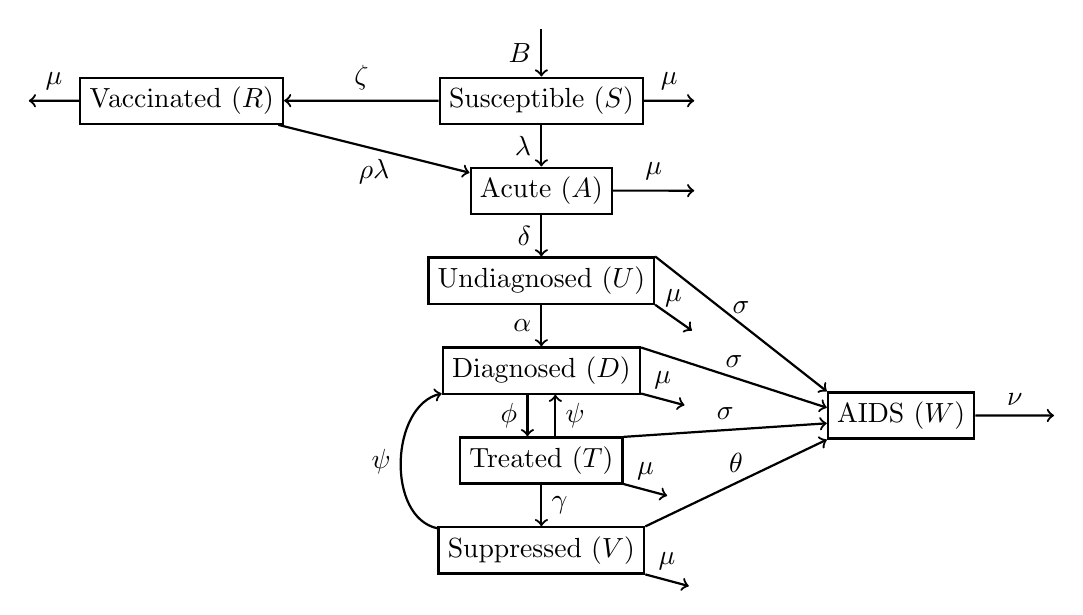
\begin{tikzpicture}[
  thick,
  scale = 1.142,
  compartment/.style = {draw},
  ]

  \node at (0, 5)
  [compartment, name = Susceptible] {Susceptible ($S$)};

  \node at (-4, 5)
  [compartment, name = Vaccinated] {Vaccinated ($R$)};

  \node at (0, 4)
  [compartment, name = Acute] {Acute ($A$)};

  \node at (0, 3)
  [compartment, name = Undiagnosed] {Undiagnosed ($U$)};

  \node at (0, 2)
  [compartment, name = Diagnosed] {Diagnosed ($D$)};

  \node at (0, 1)
  [compartment, name = Treated] {Treated ($T$)};

  \node at (0, 0)
  [compartment, name = Suppressed] {Suppressed ($V$)};

  \node at (4, 1.5)
  [compartment, name = AIDS] {AIDS ($W$)};

  \draw [->] (Susceptible) to node [left] {$\lambda$} (Acute);

  \draw [->] (Susceptible) to node [above] {$\zeta$} (Vaccinated);

  \draw [->] (Vaccinated) to node [below] {$\rho \lambda$} (Acute);

  \draw [->] (Acute) to node [left] {$\delta$} (Undiagnosed);

  \draw [->] (Undiagnosed) to node [left] {$\alpha$} (Diagnosed);

  \draw [->] (Diagnosed.240) to node [left] {$\phi$} (Treated.120);

  \draw [->] (Treated.60) to node [right] {$\psi$} (Diagnosed.300);

  \draw [->] (Treated) to node [right] {$\gamma$} (Suppressed);

  \draw [->] (Suppressed) to [out = 168, in = 193] node [left] {$\psi$} (Diagnosed);

  \draw [->] (Undiagnosed.12) to node [above] {$\sigma$} (AIDS.162);

  \draw [->] (Diagnosed.13) to node [above] {$\sigma$} (AIDS.174);

  \draw [->] (Treated.16) to node [above] {$\sigma$} (AIDS.186);

  \draw [->] (Suppressed.13) to node [above] {$\theta$} (AIDS.198);

  \draw [<-] (Susceptible) to node [left] {$B$} +(90: 0.8);

  \draw [->] (Susceptible) to node [above] {$\mu$} +(0: 1.7);

  \draw [->] (Vaccinated) to node [above] {$\mu$} +(0: -1.7);

  \draw [->] (Acute) to node [above] {$\mu$} +(0: 1.7);

  \draw [->] (Undiagnosed.348) to node [above] {$\mu$} +(325: 0.5);

  \draw [->] (Diagnosed.347) to node [above] {$\mu$} +(345: 0.5);

  \draw [->] (Treated.344) to node [above] {$\mu$} +(345: 0.5);

  \draw [->] (Suppressed.347) to node [above] {$\mu$} +(345: 0.5);

  \draw [->] (AIDS) to node [above] {$\nu$} +(0: 1.7);

\end{tikzpicture}


%%% Local Variables:
%%% mode: latex
%%% TeX-master: "model"
%%% End:

  \caption{Model diagram.}
  \label{model_diag}
\end{figure}

Our continuous-time, compartmental model consists of 8 health states:
susceptible to HIV infection, vaccinated against HIV, acute HIV
infection, undiagnosed HIV infection, diagnosed but untreated HIV
infection, treated without achieving viral suppression, achieved viral
suppression, and having AIDS (Figure \ref{model_diag}). Transitions
between states are governed by a series of differential equations
parameterized using rates estimated from other studies and from
incidence and prevalence data (Table \ref{model_param}).


\begin{table}
  \begin{center}
    \begin{tabular}{cp{4cm}llc}
      \hline
      Symbol & Definition & Value & Sampling Distribution & Source \\ \hline
      $\delta$	& Rate of leaving acute phase of HIV infection & 4.1379/year & T (4.1379, 2, 9.6) & \cite{Hollingsworth2008-iy} \\
      $\sigma$	& Rate of developing AIDS among non-virally suppressed individuals
                          & 0.1064/year & & \cite{Morgan2002-cq} \\
      $\gamma$ & Rate of viral suppression & 1/year & U (0.5, 1.5) & \cite{Currie2009-yz} \\
      $\upsilon$	& Death rate from AIDS & 0.5/year &  & \cite{Morgan2002-cq} \\
      $\omega$	& Reduction in life years for treated PLHIV & 5 & U (5, 8) & \cite{Unaids2014-ue, Samji2013-kf}\\
      $\beta_{A}$	& Transmission probability during acute phase & 0.0082 & T (0.0082, 0.0039, 0.0150) & \cite{Skarbinski2015-ni,Wawer2005-us}\\
      $\beta_{U}$	& Transmission probability after acute phase & 0.0014 & T (0.0014, 0.00077, 0.00251) & \cite{Hughes2012-so}\\
      $\varepsilon$	& Proportional reduction of transmission with treatment & 0.08 & $\beta$ (0.08, 0.002, 0.57)& \cite{Donnell2010-xo}\\
      $n$			& Sex acts per year & 102 & U (96, 108) & \cite{Wawer2005-us,Abdool_Karim2010-cm}\\ \hline
    \end{tabular}
    \caption{Parameters used in model. (T: triangular distribution, U:
      uniform distribution, $\beta$: beta distribution).}
    \label{model_param}
  \end{center}
\end{table}



The PLHIV population was comprised of people in the acutely infected,
undiagnosed, diagnosed, treated, viral suppression and AIDS
compartments. People susceptible to HIV (S) progress to the
acute-infection phase (A) according to the force of infection, which
depends on the HIV transmission rate, estimated from the
country-specific incidence and prevalence data (next section),
adjusted for the current number of acutely infected, untreated or
ineffectively treated, and viral suppression PLHIV.  Acute infection
is characterized by high viral loads and lasts 88 days on average
\cite{Hollingsworth2008-iy}. We assumed that individuals remain
undiagnosed during their acute infection phase and during at least
some of the subsequent period of clinical latency (i.e., the
undiagnosed compartment). Individuals in the undiagnosed class will be
diagnosed at a rate determined by the country's initial diagnosis
level and potential progress towards the UNAIDS targets. Diagnosed
people transition to the treated compartment upon starting ART at a
rate of $\phi$ , and to the virally suppressed class (V) after
achieving viral suppression through treatment retention at a rate of
$\gamma$. The disengagement from treatment moves individuals (T, V) at
a rate of $\omega$ back to the diagnosed class (D). Rates of movement
between the undiagnosed (U), diagnosed (D), treated (T) and virally
suppressed classes (V) are determined by the proportions of PLHIV
diagnosed ($p_{D}$), proportion of diagnosed individuals on ART
($p_{T}$), and the proportion of individuals on ART who have achieved
viral suppression ($p_{V}$). PLHIV in U, D, T, and V classes develop
AIDS (W) after an average duration dependent on viral suppression
status. Individuals who have achieved viral suppression (V) take
longer to develop AIDS ($1/\theta$), than those who are in the other
PLHIV classes ($1/\sigma$). Individuals who are susceptible to HIV can
be vaccinated at a of rate ($\zeta$), and depending on vaccine
efficacy, have a reduced chance of HIV infection. The model equations
are

\begin{equation}
  \label{model_eqns}
  \begin{split}
    \frac{\md S}{\md t} &= B N - \lambda S - \zeta S- \mu S,
    \\
     \frac{\md R}{\md t} & = \zeta S - \rho \lambda R - \mu R,
    \\
    \frac{\md A}{\md t} &= \lambda S +\rho \lambda R - \delta A - \mu A,
    \\
    \frac{\md U}{\md t} &= \delta A - \alpha U - \mu U - \sigma U,
    \\
    \frac{\md D}{\md t} &=  \alpha U + \psi T + \psi V
    - \phi D - \mu D - \sigma D,
    \\
    \frac{\md T}{\md t} &= \phi D - \psi T - \gamma T - \mu T
    - \sigma T,
    \\
    \frac{\md V}{\md t} &= \gamma T - \psi V - \mu V - \theta V,
    \\
    \frac{\md W}{\md t} &= \sigma U + \sigma D + \sigma T + \theta V -
    \nu W,
  \end{split}
\end{equation}
with force of infection
\begin{equation}
  \label{force_of_infection}
  \begin{split}
    \lambda &= \frac{\beta_A A + \beta_U (U + D + T) + \beta_T V}{N},
    \\
    N &= S + R +  A + U + D + T + V,
    \\
    \beta_x &= c \left[1 - (1 - \tau_x)^n\right]
    \text{ for $x \in \{A, U, T\}$},
    \\
    \tau_T &= (1 - \epsilon) \tau_U.
  \end{split}
\end{equation}

The rate of developing AIDS  among those who have acheived
viral suppression ($\theta$) is
\begin{equation}
 \frac{1}{1/\mu-\omega-1/\nu}.
\end{equation}

The proportion diagnosed is
\begin{equation}
  p_D = \frac{D + T + V + W}{A + U + D + T + V + W},
\end{equation}
the proportion treated is
\begin{equation}
  p_T = \frac{T + V + W}{D + T + V + W},
\end{equation}
and the proportion with viral suppression is
\begin{equation}
  p_V = \frac{V}{T + V}.
\end{equation}

The targets for the proportions $p_D$, $p_T$, and $p_V$ in the achievement of 90--90--90
all operate under the following assumption:
if the initial level $p_x(0)$ is less than $90\%$, the proportion will increase
linearly in the first 5 years and then stay at $90\%$ for the
remaining time; and if the initial level is at $90\%$ or above, the proportion
will remain constant for the duration of the study:
\begin{equation}
  p_x^*(t)
  = p_x(0) + \left[
    \max\left\{0.9, p_x(0)\right\} - p_x(0)
  \right]
  \min\left\{\frac{t}{5}, 1\right\},
\end{equation}
for $x \in \{D, T, V\}$.

Similarly, the proportion of people vaccinated is
\begin{equation}
P_{V} = \frac{R}{S+R},
\end{equation}

We can implement the vaccination compartment in the same way as the other controls. When we begin
vaccination in 2020/2025, the initial vaccination level is 0\%. This
coverage will increase linearly to $50\%$ within first 2 or 5
years. The coverage will continue to increase linearly till it reaches
the desired coverage ($50\%,70\%,90\%$) and then stay constant for the
remainder of the projections.

95--95--95 goal is implemented subsequently after meeting 90--90--90
by 2020 by increasing $p_D$, $p_T$, and $p_V$ to 95--95--95 levels by
2030 linearly. \comment{@Jan, We use the Heaveside function here too?}


\subsection{Rates that are on when $p_x < p^*_x$}

The rates are applied when the proportions of $p_D$, $p_T$, and $p_V$ are below the target levels:
\begin{equation}
  \begin{split}
    \alpha(t) &= \alpha_{\max} H\left(p_D^*(t) - p_D(t)\right),
    \\
    \phi(t) &= \phi_{\max} H\left(p_T^*(t) - p_T(t)\right),
    \\
    \psi(t) &= \psi_{\max} H\left(p_V(t) - p_V^*(t)\right),
    \\
    \zeta(t) &= \zeta_{max} H\left(P^{*}_{V}(t)-P_{V}(t)\right),
  \end{split}
\end{equation}
where $H(x)$ is the Heaviside function
\begin{equation}
  H(x) =
  \begin{cases}
    0 & \text{if $x < 0$},
    \\
    1 & \text{if $x > 0$}.
  \end{cases}
\end{equation}

The discontinuity of the Heaviside function makes numerical solution
difficult.  Instead, replace $H$ with the continuous piecewise linear
function
\begin{equation}
  H(x) =
  \begin{cases}
    0 & \text{if $x < 0$},
    \\
    x / \chi & \text{if $0 \leq x \leq \chi$},
    \\
    1 & \text{if $x > \chi$},
  \end{cases}
\end{equation}
with some small value of $\chi$.


\section{Model fitting}
\label{model_fitting}
We first estimated country-specific rates of HIV transmission for each
of the available historical data point for incidence and
prevalence. The calculation involved a simplified force of infection
that initially assumed no differences in transmission risk among
acute, unsuppressed, suppressed, and AIDS classes due to the general
lack of historical data on diagnosis and treatment. We calculated a
time-independent aggregate transmission rate by taking an exponential
weighted mean of the historical (i.e., time-dependent) transmission
rates for each given country (\autoref{transmission_rate}). The
aggregate transmission rate was then combined with estimated HIV
transmission risk by stage of HIV infection
\cite{Hollingsworth2008-iy} and treatment status \cite{Wawer2005-us}
to calculate separate transmission rates for unsuppressed, acute, and
viral-suppression people. These rates were used to simulate model
projections through 2035.



{We calibrated longitudinal HIV incidence and prevalence data from
  1990 to 2015 incidence in addition to data on $p_{D}$, $p_{T}$ and
  $p_{V}$ levels in 2015 to estimate the rate of transmission for each
  country. The calculation involved a simplified force of infection:}

\begin{align}
  \label{foi}
  \begin{split}
  \lambda(t) &  =    \frac{\beta_{A} A + \beta_{U}(U+D+T)+\beta_{V}V+0
               W}{N} \\
             &  =  \beta \frac{I}{N},
             \end{split}
\end{align}
where $\beta$ is the estimated time-independent aggregate transmission rate under the
assumption that there is no difference in transmission risk among acute, unsuppressed, suppressed, and AIDS classes.

$I = A+U+D+T+V+W$ is the total number of people living with HIV. Therefore, the per-capita
incidence is
\begin{equation}
i(t) = \lambda(t) \frac{S(t)}{N(t)}
= \beta(t) \frac{I(t)}{N(t)} \frac{S(t)}{N(t)} =\beta(t) p(t) (1-p(t)),
\end{equation}
where $p(t)$ is the prevalence. Thus, we can estimate the
transmission rate at each historical time point using the incidence
and prevalence data,
\begin{equation}
  \label{trans_rate}
  \beta(t) = \frac{i(t)}{p(t)(1-p(t))}
\end{equation}


We estimated the time-independent aggregated transmission rate ($\beta$)
by taking the exponential weighted mean of transmission rates
(\ref{trans_rate}).


Rearranging equation (\ref{foi}), the transmission rate for PLHIV
without viral suppression can be written as
\begin{equation}
\label{betaU}
  \beta_{U} = \frac{\beta I}{\frac{\beta_{A}}{\beta_{U}}A +
    U+D+T+\frac{\beta_{V}}{\beta_{U}}V}
\end{equation}


Next, we assumed that the relative risk of acute HIV transmission
($\beta_{AU} = \beta_{A}/\beta_{U}$) and virally suppressed HIV
transmission ($\beta_{VU} = \beta_{V}/\beta_{U}$) with respect to the
unsuppressed transmission remains constant worldwide and calculated
these values using the data from Rakai, Uganda \cite{Wawer2005-us}. The aggregate
rate of transmission ($\beta$) can then be combined with equations \ref{betaU} to calculate transmission
rates for unsuppressed PLHIV, acute PLHIV and suppressed PLHIV as,
\begin{align}
  \beta_{U} & = \frac{\beta I}{\beta_{AU}A +
              U+D+T+\beta_{VU}V}, \\
  \beta_{A} & = \beta_{AU}\beta, \\
  \beta_{V} & = \beta_{VU} \beta.
\end{align}
that we use to simulate our model forward and project results up to 2035.
\\

\comment{Need to add stuff about how we generate distribution of
  transmission rates}




\begin{figure}
  \centering
  \includegraphics[width = \textwidth]{../Codes/plots/transmission_rate}
  \caption{Country-specific transmission rates were calculated based
    on the relative contributions of individuals with acute infection,
    unsuppressed viral load or suppressed viral load to overall
    transmission (\autoref{model_fitting}). The estimates were
    calibrated to data on country-level incidence and/or prevalence to
    account for variation in historical incidence while accurately
    reflecting recent HIV rates.}
  \label{transmission_rate}
\end{figure}


\section{Analysis}

We evaluated the global and country-specific impacts of meeting the
UNAIDS targets and vaccine deployment on four outcome measures: HIV
incidence, PLHIV, number of people with AIDS, and AIDS-related deaths
between 2015 and 2035. Calibrating our model to historical data on
prevalence and incidence, we projected the anticipated trajectories of
the outcomes using country-specific transmission rates across the
intervention scenarios outlined below.  Our base-case scenario assumed
maintenance of the status quo: that 2015 levels of the proportion of
PLHIV diagnosed ($p_{D}$), proportion of those diagnosed on ART
($p_{T}$), and proportion of those on treatment who have achieved
viral suppression ($p_{V}$) continue unchanged until 2035.  The
intervention scenarios were (1.) the attainment of the 90--90--90
target by linear increases in $p_{D}$, $p_{T}$, and $p_{V}$ until 2020
followed by maintenance of those levels until 2035, and (2.) linear
increase in the diagnosis and treatment levels to the 90--90--90
targets by 2020, a linear increase from 90--90--90 to the 95--95--95
target by 2030, and maintenance of the 95--95--95 levels to 2035. (For
90--90--90, if any initial level was above 90\%, it was kept constant
going forward so that the intervention did not worsen coverage.
Likewise, for 95--95--95, any initial level above 95\% was kept
constant.)  For vaccination, we assumed deployment of a vaccine with
50\% efficacy in 2020 with coverage increasing linearly from 0\% to
50\% at 2 years post-rollout and maintaining constant coverage after
reaching 70\%. The added benefit of vaccination was considered in the
context of status quo diagnosis and treatment, achieving the UNAIDS
90–90–90 goal by 2020 followed by maintenance, and achieving the
95–95–95 goal by 2030 followed by maintenance.  Projections were
generated through model simulations based on published parameter
distributions (\autoref{model_param}) and country-specific estimated
transmission rate distributions. The parameters were sampled using
latin hypercube sampling \cite{}
and the variance reduction technique of running different
interventions with random parameter values \cite{}.

We calculated partial rank correlation coefficients (PRCC) to measure
the independent effect of each parameter on model projections of HIV
incidence (\autoref{PRCCs}). Furthermore, due to uncertainty
surrounding the prospective vaccine, we obtained model projections
using six additional vaccine scenarios by considering alternative
estimates of efficacy (30\%, 70\%), coverage (50\%, 90\%), time to
50\% coverage (2 years, 5 years), and first year of availability
(2025).

\begin{figure}
  \centering
  \includegraphics{../Codes/plots/prcc.pdf}
  \caption{Parameter sensitivity of model global infections averted
    from 2015 to 2035.}
  \label{PRCCs}
\end{figure}


\subsection{Effectiveness of HIV interventions globally, regionally
  and for each of 127 countries}

Model outcomes were projected until 2035 for each of the 127 countries
with sufficient data on status quo rates of diagnosis and treatment
and on historical incidence or prevalence. The median estimates with
interquartile ranges are presented between 2015 and 2035 for number of
PLHIV, annual incidence (per million population), number of people
with AIDS, and number of HIV-related deaths under the status quo and
five intervention scenarios: vaccination only, attainment of the
UNAIDS 90--90--90 target, 90--90--90 target and vaccination, attainment of
the UNAIDS 95--95--95 target, and 95--95--95 target and vaccination.  The
country-specific projections as well as aggregated projections at the
regional and global levels follow:


\bibliographystyle{science_nat}

\bibliography{supplementary_text}


\clearpage
\input{../Codes/plots/effectiveness_all/all}


\end{document}
